\documentclass[12pt, oneside, a4paper, svgnames]{book}

\usepackage{array}
\usepackage[boxruled, linesnumbered]{algorithm2e}
\usepackage{amsmath}
\usepackage{amssymb}
\usepackage{amsthm}
\usepackage[toc]{appendix}
\usepackage{biblatex}
\usepackage{bm}
\usepackage{booktabs}
\usepackage{etoolbox}
\usepackage{fancyhdr}
\usepackage[T1]{fontenc}
\usepackage[a4paper, top=25.4mm, bottom=25.4mm, right=25.4mm, left=40mm]{geometry}
\usepackage{graphicx}
\usepackage{hyperref}
\usepackage{istgame}
\usepackage{kbordermatrix}
\usepackage{listings}
\usepackage{mathtools}
\usepackage{minted}
\usepackage{multirow}
\usepackage[parfill]{parskip}
\usepackage{subcaption}
\usepackage{tikz}
\usepackage{xcolor}



\linespread{1.25}

\fancypagestyle{normal}{
	\fancyhf{}
	\fancyhead[L]{\slshape \leftmark}
	\fancyhead[R]{\thepage}
	\renewcommand{\headrulewidth}{0pt}
}

\fancypagestyle{chapterstyle}{
	\fancyhf{}
	\fancyhead[R]{\thepage}
	\renewcommand{\headrulewidth}{0pt}
}


\patchcmd{\chapter}{\thispagestyle{plain}}{\thispagestyle{chapterstyle}}{}{}



\renewcommand{\kbldelim}{(}
\renewcommand{\kbrdelim}{)}


\renewcommand\arraystretch{1.5}
\renewcommand{\tabcolsep}{0.5cm}

\graphicspath{{images/}}



\addbibresource{{tex/references/main.bib}}


\theoremstyle{definition}
\newtheorem{definition}{Definition}[section]

\newtheorem{theorem}{Theorem}[section]


\usetikzlibrary{snakes}
\usetikzlibrary{positioning}


\begin{document}

\newgeometry{a4paper, top=25.4mm, bottom=25.4mm, right=25.4mm, left=25.4mm}
\begin{titlepage}
	\begin{center}
		\vspace*{0.5cm}
		
\includegraphics[width=5cm]{cardiff-uni-logo.jpg}

		\vspace{1cm}

		\huge
		An Empirical Study on the Folk Theorem

		\vspace{2cm}

		\large
		Student: Sophie Shapcott

		\vspace{0.5cm}

		Supervisor{(s)}: Dr Vince Knight and Henry Wilde 

		\vspace{0.5cm}

		Academic Year: 2019/20
		
		\vspace{0.5cm}

		School of Mathematics, \\Cardiff University

		\vfill

		\normalsize
		A final year undergraduate project submitted in partial fulfilment of the\\ requirements for MMORS (Masters in Mathematics, Operational Research\\ and Statistics) taught programme.

	\end{center}
\end{titlepage}

\restoregeometry

\frontmatter
\pagestyle{chapterstyle}
\chapter{Summary}

This project consists of an empirical study into a class of theorems, entitled
`Folk Theorems', which are a key part of the repeated games theory. The aims of
the project include: an in-depth review of academic literature regarding the
topic; the development and execution of a large experiment based on the
`original' folk theorem of Friedman~\cite{Friedman1971} with the Iterated
Prisoner's Dilemma; and an analysis of the effects of different tournament
characteristics on the \(p\)-threshold appearing in the folk theorems. These
ideas are extended from a third year assignment in Game Theory, completed by the
author.

Firstly, after an introduction to the theory of one-shot and repeated games, a
search of the folk theorem literature is provided in Chapter~\ref{ch:Lit_Review}. This reveals the vast
directions of research in the area for the past fifty years. Many
generalisations and refinements of the folk theorem have been analysed since the
first written papers in the 1970s. The games for which the notion has been
expanded to range from complete information games to games with imperfect
private monitoring. However, in certain cases, the strategies used in the proof
of these are unstable. Also, in situations where an individual deviator cannot
be identified, a much smaller set of payoffs can be achieved, yielding the
so-called `Anti-Folk Theorems'. More recently, focus has been on the application
of the folk theorem to computing and quantum transportation, for example.
Finally, it is concluded that, to the best of the author's knowledge, this is
the fist study to execute an experiment on the folk theorem of this size.

Following this, a detailed description of how the experiment was set-up and
executed is provided in Chapter~\ref{ch:Methods}, with justifications to the specific methods and software
chosen. After considering the benefits and drawbacks of varying file formats for
storing data, it is stated that a relational database, in particular SQLite,
would be the most appropriate. This is due to: the existence of libraries in
Python enabling the easier access of the data; the general robustness of
databases; and its ability to perform out of memory operations. Due to the
pre-existing game theoretic libraries, Axelrod and Nashpy, Python was chosen as
the language of implementation and ensuring good software development principles
were followed is highlighted as a priority. The volume of data which was planned
to be collected meant that remote computing was required and is explained in
this chapter. Here, the choice of support enumeration for the calculation of
Nash equilibria and the potential issues which may be faced due to degeneracy is
also discussed.

The main analysis of the data collected is provided in
Chapter~\ref{ch:Analyses}. An initial analysis discussing the characteristics of
the strategies used and the overall summary statistics is detailed, before the
\(p\)-thresholds are explored. The characteristics of tournaments focused on
are: the number of opponents the Defector had and the level of tournament noise
included. However, this is concluded as a non-trivial task due to the
uncertainty regarding the degeneracy of a large proportion of tournament sets.
Also, the inevitability of randomness within the tournaments meant that a lot
more data than what was obtained is required. On the other hand, the graphs that
were yielded are stated as successful in visualising the folk theorem.

Finally, Chapter~\ref{ch:Conclusions_and_Recommendations} details the
conclusions of the research before giving recommendations for further work.
Amongst these were suggestions on how more characteristics of the tournament set
could be studied as well as the potential to predict the \(p\)-threshold from
the characteristics of the tournaments via regression analysis.
\chapter{Acknowledgements}

First and foremost, I would like to express my sincere thanks and gratitude to
my project supervisors Dr Vince Knight and Henry Wilde for their continual
advice, support and invaluable ideas throughout the completion of this project.
You have always been willing to lend a hand or provide encouragement when
it was needed the most. You have assisted me
through what will probably be the largest project I will ever complete!

There are many people who have helped and supported me, both inside and outside
university, over the past four years of my undergraduate degree here at Cardiff
School of Mathematics. If I was to mention all the names, this would be longer
than my whole project! Therefore, this `thank you' is for all those who I have
had the pleasure of being taught by and working with during my degree. You have
made this journey an interesting and enjoyable one and I will continue to be
inspired by the passion all the lecturers have for what they do. 

Also, I would like to give special mention to Nikoleta, who, even though is in
her final few months of a PhD, found time
to talk and make sure I was still operating on this planet. You
encouraged me and always had a positive thing to say when I was convinced
everything was going to end terribly. So thank you very much for being
such a great friend and best of luck with the completion of your thesis.

Last but most certainly not least, I want to say a huge thank you to my Mum, Dad
and Zoe for their continual love and support. To say these have been a
challenging four years is an understatement. My
Mum, thank you for keeping me fuelled with coffee and biscuits through the long
days and for being a shoulder to cry on when necessary. I will give you enough
hair dye to cover all those grey ones I caused! Dad, thank you for making me
laugh with your terrible jokes, and finally Zoe, (yes, you are
getting a mention because, yes, you did play a key part) thank you for keeping
me sane and being a great sister.

To those I have forgotten to mention: my apologies and thank
you.

\tableofcontents
\listoffigures

\mainmatter
\pagestyle{normal}

\chapter{Introduction}\label{ch:Introduction}
World War I, a time of harsh conflict and battle, provided an example of how
cooperation need not evolve from friendship. Indeed,~\cite{Axelrod1984a} states
that small units of common soldiers on the Western Front were able to execute a
``live and let live'' system, even against the will of the officers. They knew
that ``if the British shelled the Germans, the Germans replied; and the damage
was equal'' (quoted from~\cite{Cobb1916} as given in~\cite{Axelrod1984a}).
Moreover, this was achieved without a direct truce as officers forbade it. The
analysis of such circumstances, and other situations involving choice, is
covered by an area of mathematics entitled \textit{game theory}.

According to~\cite{Dictionary2013}, \textit{game theory} is the study of interactive
decision making and the development of
strategies through mathematics. It analyses and gives
methods for predicting the choices made by players (those making a decision),
whilst also suggesting ways to improve their
`outcome'~\cite{maschler_solan_zamir_2013}. Here, the abstract notion of utility
is the outcome players wish to maximise. For further information on the topic of
utility theory, readers are referred to Chapter 2
in~\cite{maschler_solan_zamir_2013} for a detailed discussion or Section
1.3 in~\cite{Webb2007} for a more introductory explanation. 

One of the earliest pioneers of game theory is mathematician, John von Neumann
who, along with economist Oskar Morgenstern, published \textit{The Theory of
Games and Economic Behaviour} in 1944~\cite{maschler_solan_zamir_2013}. This
book~\cite{von2007theory} discusses the theory, developed in 1928 and 1940, by von Neumann,
regarding ``games of strategy'' and its applications within the subject of
economics. Following this, several advancements have been
made in the area including, most notably, John Nash's papers on the
consequently named
Nash Equilibria in 1950-51~\cite{nash1951non, nash1950equilibrium}. Due to the
``context-free mathematical toolbox''~\cite{maschler_solan_zamir_2013} nature of
this subject, it has been applied to many areas, from
networks~\cite{liang2012game, 1593279} to biology~\cite{adeoye2012application, chen2009robust}. 

In this project, the main focus is a
class of theorems within game theory, known as ``Folk Theorems''. These ideas
assist in the analysis of long-term behaviour and evolution of cooperative
strategies. In particular, the theory will be applied to the game of a
Prisoner's Dilemma which is introduced in subsequent sections. The structure of
this report is as follows: Chapter~\ref{ch:Lit_Review} provides a literature review
on the topic of folk theorems, before Chapter~\ref{ch:Methods} discusses the
development of a large experiment regarding these notions in the Prisoner's
Dilemma. Chapter~\ref{ch:Analysis} analyses the results obtained
whilst Chapter~\ref{ch:Conclusions} provides the conclusions and recommendations for
further study. However, first, the remainder of Chapter~\ref{ch:Introduction} is dedicated
to the key definitions and theorems required for a study in game theory.

Unless stated otherwise, the definitions and notation in this chapter have been
adapted from~\cite{maschler_solan_zamir_2013}.

\section{An Introduction to Games}\label{sec:An_Intro_to_Games}
Consider the following scenario:

\begin{center}
    Two convicts have been accused of an illegal act. Each of these prisoners,
    separately, have to decide whether to reveal information (defect) or stay
    silent (cooperate). If they both cooperate then the convicts are given a
    short sentence whereas if they both defect then a medium sentence awaits.
    However, in the situation of one cooperation and one defection, the prisoner
    who cooperated has the consequence of a long term sentence, whilst the other
    is given a deal~\cite{Knight2017, maschler_solan_zamir_2013}.
\end{center}

This is one of the standard games in game theory known as the Prisoner's
Dilemma (PD). It has four distinct outcomes, for the given two player version,
which can be viewed in Table~\ref{tab:PD_outcomes}. Note, following the standard
literature, cooperation and defection is indicated by \(C\) and \(D\), respectively.

\begin{table}
    \centering
    \begin{tabular}{c|c}
        \(C, C\) & \(C, D\) \\
        \midrule
        \(D, C\) & \(D, D\) \\
    \end{tabular}
    \caption{Outcomes for a game of the Prisoner's Dilemma.}\label{tab:PD_outcomes}
\end{table}

More formally, the game can be represented as the following matrix:
\begin{equation}
    \kbordermatrix{
        \mbox{ } & C & D\\ 
        C & (3, 3) (R, R) & (0, 5) (S, T)\\ 
        D & (5, 0) (T, S) & (1, 1) (P, P)
    }
\end{equation}\label{eqn:PDMatrix}
where each coordinate \((a, b)\) in the table represents the utility values
obtained for each player, where \(a\) is the utility value obtained by the row
player and \(b\) is the utility gained by the column player. These utility
values (payoffs)\footnote{`Utility' is referred to as a player's `payoff'
throughout the remainder of this report.} are as given
in~\cite{axelrod1980effective} and
used throughout this project. In general, the PD payoffs are constrained by the
two conditions:

\begin{equation}
    T > R > P > S
\end{equation}\label{eqn:PD_1}
and
\begin{equation}
    2R > T + S
\end{equation}\label{eqn:PD_2}

where~\eqref{eqn:PD_1} ensures that \(D\) is preferable to \(C\) and
yet~\eqref{eqn:PD_2} ensures that mutual \(C\) is
best~\cite{Knight2019,Press2012}. The matrix given in~\eqref{eqn:PDMatrix} is
known as a \textit{normal form} representation of the game.

\begin{definition}
    In general a \textit{normal form} or \textit{strategic form} game is defined
    by an ordered triple \(G = (N, {(S_i)}_{i \in N}, {(u_i)}_{i \in N})\), where:
    \begin{itemize}
        \item \(N = \{1, 2,\ldots, n\} \) is a finite set of players;
        \item \(S = S_1 \times S_2, \times \cdots \times S_n\) is the set of
        strategies for all players in which each vector \({(S_i)}_{i \in N}\) is
        the set of strategies for player \(i\)\footnote{Since the game of the PD has a finite strategy set for each player \(S_i=\{\text{C},
        \text{D}\} (i = 1, 2, \ldots, n)\), in this project only finite
        strategy spaces are considered.}; and
        \item \(u_i : S \to \mathbb{R}\) is a payoff function which associates each
        strategy vector, \(s = {(s_i)}_{i \in N}\), with a utility
        \(u_i(i \in N)\).
    \end{itemize}
\end{definition}

Yet another way of representing this game is as a pair of matrices, \(A, B\),
defined as follows:
\begin{equation}
    A = 
    \begin{pmatrix}
       3 & 0\\
       5 & 1\\ 
    \end{pmatrix}
    \text{ and } B = A^{T} =
    \begin{pmatrix}
        3 & 5\\
        0 & 1\\
    \end{pmatrix}
\end{equation}
This way of defining games allows for the use of linear algebraic expressions in
the calculation of utilities (see Section~\ref{sec:NE_for_Normal_Form_Games}).

Before continuing the discussion into the key notions of game theory, it needs
to be highlighted that there is an important assumption, which is central to
most studies of game theory, entitled \textit{Common Knowledge of Rationality}.
This, more formally, is a recurring list of beliefs which claim:
    \begin{itemize}
        \item The players are rational;
        \item All players know that the other players are rational;
        \item All players know that the other players know that they are 
        rational; 
        \item etc.    
    \end{itemize}
Assuming Common Knowledge of Rationality allows for the prediction of rational
behaviour through a process known as \textit{rationalisation}
~\cite{Knight2019}. See Section 4.5 in~\cite{maschler_solan_zamir_2013} for an
alternative explanation of this assumption. 

Thus far, only the pure strategies, \(S_{i}=\{C, D\} \), have
been discussed, hence the notion of a probability distribution over \(S_{i}\) is
now introduced, giving the so-called \textit{mixed strategies}.

\begin{definition}
   Let \(G=(N, {(S_{i})}_{i \in N}, {(u_{i})}_{i \in N})\) be a game, then a \textit{mixed strategy} for player \(i\) is a
probability distribution over their strategy set \(S_{i}\). The set of mixed
strategies for player \(i\) is defined by 
\begin{equation}
    \Sigma_{i} = \left \{ \sigma_{i} : S_{i} \to [0, 1] \mid \sum_{s_{i} \in S_{i}}{\sigma_
{i}(s_{i})} = 1 \right \}. 
\end{equation}
\end{definition}

Hence, observe that the pure
strategies are specific cases of mixed strategies, with \(\sigma_{i} = (1, 0)\)
for cooperation and \(\sigma_{i} = (0, 1)\) for defection, in the PD\@.

This leads onto the following definition of a \textit{mixed extension} for a
game.

\newpage
\begin{definition}
    Let \(G\) be a finite normal form game as above, with \(S = S_{1} \times
S_{2} \times \cdots \times S_{n}\) defining the pure strategy vector set and
each pure strategy set, \(S_{i}\) being non-empty and finite. Then the
\textit{mixed extension} of \(G\) is denoted by
\begin{equation}
    \Gamma = (N, {(\Sigma_{i})}_{i \in N}, {(U_{i})}_{i \in N}), 
\end{equation}
and is the game in which, \(\Sigma_{i}\) is the \(i\)th player's strategy set
and \(U_{i} : \Sigma \to \mathbb{R}\) is the corresponding payoff function,
where each \(\sigma = (\sigma_{1}, \sigma_{2}, \ldots, \sigma_{n}) \in \Sigma =
\Sigma_{1} \times \Sigma_{2} \times \cdots \times \Sigma_{n}\) is mapped to the
payoff:
\begin{equation}
    U_{i} = \mathbb{E}_{\sigma}(u_{i}(\sigma)) = \sum_{(s_{1}, s_{2}, \ldots, s_
    {n}) \in S}{u_{i}(s_{1}, s_{2}, \ldots, s_{n})\sigma_{1}(s_{1})\sigma_{2}(s_
    {2})\cdots\sigma_{n}(s_{n})} 
\end{equation}\label{eqn:mixed_payoff_function}
for all players \(i \in N\).
\end{definition}

\section{Nash Equilibrium for Normal Form Games}\label{sec:NE_for_Normal_Form_Games}
As mentioned above, mathematician, John Nash, introduced the concept of an
equilibrium point and proved the existence of mixed strategy Nash Equilibria in
all finite games. These notions are central to the study of game
theory~\cite{maschler_solan_zamir_2013} and hence, in this section, Nash's
concepts will be defined and proved in detail.

Firstly, the idea of a \textit{best response} is introduced.
\begin{definition}
    For a game \(G=(N, {(S_{i})}_{i \in N}, {(u_{i})}_{i \in N})\), the strategy,
\(s_{i}\), of the \(i\)th player is considered a \textit{best response} to the
strategy vector \(s_{-i}\) if \(u_{i}(s_{i}, s_{-i}) = \max_{t_{i} \in
S_{i}}u_{i}(t_{i}, s_{-i})\).
\end{definition}

This leads onto the main definition of the section.
\begin{definition}
    Given a game \(G=(N, {(S_{i})}_{i \in N}, {(u_{i})}_{i \in N})\) and its
    mixed extension, \(\Gamma \), the vector of
    strategies \(\sigma^{*} = (\sigma_{1}^{*}, \sigma_{2}^{*}, \ldots, \sigma_{n}^{*})\) is a
    \textit{Nash equilibrium} if, for all players \(i \in N\), \(\sigma_{i}^{*}\) is 
    a best response to \(\sigma_{-i}^{*} \in N\).
\end{definition}\label{def:NE}

In other words, \(\sigma^{*}\) is a Nash equilibrium if and only if no player has any
reason to deviate from their current strategy \(\sigma_{i}^{*}\).

The following observation is highlighted as an example.

\begin{center}
    \textbf{The strategy pair \((D, D)\), is the unique Nash equilibrium 
    for the PD, with a payoff value of 1 for each player.}
\end{center}

Assume the row player uses the following mixed strategy, \(\sigma_{r} = (x,
1-x)\), that is, the probability of cooperating is \(x\) and the probability of
defecting is \(1-x\). Similarly, assume the column player has 
the strategy, \(\sigma_{c} = (y, 1-y)\). The payoff obtained for the row and column player, respectively, is then:
\[
    A\sigma_{c}^T = \begin{pmatrix}
        3 & 0 \\
        5 & 1
    \end{pmatrix} \begin{pmatrix}
        y \\
        1-y
    \end{pmatrix} = \begin{pmatrix}
        3y \\
        4y + 1
    \end{pmatrix},
\]
\[
    \sigma_{r}B = \begin{pmatrix}
        x & 1-x
    \end{pmatrix} \begin{pmatrix}
        3 & 5 \\
        0 & 1        
    \end{pmatrix}  = \begin{pmatrix}
        3x & 4x + 1
    \end{pmatrix}.
\]

Plotting these gives the graphs as seen in Figure~\ref{fig:mixed_strategy_PD}.

\begin{figure}
    \centering
    \begin{subfigure}{0.45\textwidth}
        \centering
        \includegraphics[width=\textwidth]{{pd-row-payoff}}
    \end{subfigure}
    \begin{subfigure}{0.45\textwidth}
        \centering
        \includegraphics[width=\textwidth]{{pd-col-payoff}}
    \end{subfigure}
    \caption{Graphs to show the row and column players' payoffs against a 
    mixed strategy.}\label{fig:mixed_strategy_PD}
\end{figure}

From Figure~\ref{fig:mixed_strategy_PD} it is clear that, regardless of the
strategy played by the opponent, defection is indeed the only rational move. Thus, the players have no incentive to deviate if and only if both
play the strategy \(\sigma=(0, 1)\), that is, defection for every one-shot game
of the PD\@.

This next result is taken from~\cite{nash1951non}, Nash's second paper on
equilibria in games. The notion obtained here is fundamental to many areas of
game theory, including the folk theorems.

\begin{theorem}
    Every finite game has an equilibrium point.
\end{theorem}\label{thm:Nash}

The proof of Theorem~\ref{thm:Nash} includes the use of a \textit{fixed point
theorem}. Thus, a short sub-section regarding one such result is given for
completeness, before providing a formal proof of Theorem~\ref{thm:Nash}.

\subsection{Brouwer's Fixed Point Theorem}\label{subsec:Brouwer_thm}
Brouwer's Fixed Point Theorem is a result from the field of topology. Named
after the Dutch mathematician, L.E.J. Brouwer, it was proven in
1912~\cite{Carlson2016}. However, before stating this notion, a few conditions
regarding the properties of sets are recalled. 

The following three definitions appear as 
in~\cite{Barile,Weissteina,Weisstein}
for Definitions~\ref{def:open_cover},~\ref{def:compact}, and~\ref{def:convex}, respectively.

\begin{definition}
    A set \(X \subseteq \mathbb{R}^{d}\) is called \textit{convex} if it
    contains all line segments connecting any two points \({x}_{1},
    {x}_{2} \in X\).
\end{definition}\label{def:convex}

\begin{definition}
    An \textit{open cover} of a set \(S \subset X\), a topological space, is a
    collection of open sets \(A_{1}, A_{2}, \ldots \subset X\) such that
    \(A_{1} \cup A_{2} \cup \ldots \supset S\), that is, the union of the open
    sets contain S.
\end{definition}\label{def:open_cover}

\begin{definition}
    A subset \(S \subseteq X\), a topological space, is called \textit{compact}
    if, for each open cover of \(S\), there is a finite sub-cover of S.
\end{definition}\label{def:compact}

The presentation of Brouwer's Fixed Point Theorem is now given as 
in~\cite{maschler_solan_zamir_2013}.

\begin{theorem}
    Let \(X \subseteq \mathbb{R}^{n}\) be a non-empty convex and compact
    set, then each continuous function \(f : X \to X\) has a fixed point.  
\end{theorem}\label{thm:Brouwer}

In other words if \(X\) and \(f\) satisfy the conditions given above then there
exists a point \(x \in X\) such that \(f(x) = x\). 

Since this project is regarding game theory, rather than topology, the proof to
the above theorem is omitted. However, the interested reader is referred
to~\cite{Henle1979} for an in-depth consideration into the theory of topology.

\subsection{Proof of Nash's Theorem}\label{subsec:Nash_Proof}
The proof provided is adapted from the original, as presented
in~\cite{nash1951non}, with extra notes from~\cite{maschler_solan_zamir_2013}.
According to~\cite{maschler_solan_zamir_2013}, the general idea is to
define a function, which satisfies the conditions required
for Theorem~\ref{thm:Brouwer}, by using the payoff functions on the set of mixed
strategies. Then, through identifying
each equilibrium point with a fixed point of the function, the required result 
is obtained.

Firstly, a brief restatement of the notation needed is provided for clarity.
Let \(G=(N, {(S_{i})}_{i \in N}, {(u_{i})}_{i \in N})\) be a finite game with
mixed extension \(\Gamma=(N, {(\Sigma_{i})}_{i \in N}, {(U_{i})}_{i \in N})\).
Here, \(N = \{1, \ldots, n\} \) denotes the set of players; \(S = S_{1} \times S_{2} \times
\ldots \times S_{n}\) is the set of pure strategies for all players, with
\({(S_i)}_{i \in N}\) the pure strategy set for player i; \(\Sigma \) is
defined similarly but relating to mixed strategies; and \(U_{i}: \Sigma \to
\mathbb{R}\) are the payoff functions as given in~\eqref{eqn:mixed_payoff_function}.

\begin{proof}
    Let \(\sigma = (\sigma_{1}, \sigma_{2}, \ldots, \sigma_{n})\) be a tuple of
    mixed strategies and \(U_{i,t}(\sigma)\) be the \(i\)th player's payoff if
    they changed to their \(s_{i}^{t}\)th pure strategy and all other players
    continue to use their mixed strategy.
    Now, define function \(f: \Sigma \to [0, \infty)\) such that 
    \begin{equation}
        f_{i,t}(\sigma) = \max{(0, U_{i,t}(\sigma)-U_{i}(\sigma))}
    \end{equation}
    and also let 
    \begin{equation}
        \sigma_{i}^{\prime} = \frac{ \sigma_{i}+\sum_{t}{f_{i,t}(\sigma)s_{i}^{t}} }{ 1+\sum_{t}{f_{i,t}(\sigma)} }
    \end{equation}
    be a modification of each \(\sigma_{i} \in \sigma \), with \(\sigma^{\prime}
    = (\sigma_{1}^{\prime}, \sigma_{2}^{\prime}, \ldots, \sigma_{n}^{\prime})\).
    In words, this modification increases the proportion of the pure strategy
    \(s_{i}^{t}\) used in \(\sigma_{i}\) if the payoff gained by the \(i\)th player is
    larger when they replace their mixed strategy by \(s_{i}^{t}\). Else, it remains the
    same if doing this decreases their payoff as \(f_{i,t}(\sigma)=0\) in this
    case. Note, the denominator ensures that the ending vector is still a
    probability distribution by standardising.

    The aim is to apply Theorem~\ref{thm:Brouwer} to the mapping \(T: \sigma \to
    \sigma^{\prime}\) and show that its fixed points correspond to Nash
    equilibria. Thus, firstly compactness and convexity of the set \(\Sigma \)
    is shown along with continuity of the function \(f\). 
    
    \textbf{Claim 1: The set \(\Sigma \) is compact and convex.}
    Observe that each \(\sigma_{i}\) can be represented by a point in a simplex
    in a real vector space with the vertices given by the pure strategies,
    \(s_{i}^{t}\). Therefore, it follows that the set \(\Sigma_{i}\) is convex
    and compact. Using the result, \textit{If \(A \subseteq \mathbb{R}^{n}\) and
    \(B \subseteq \mathbb{R}^{m}\) are convex compact sets then the set \(A
    \times B\) is a convex compact subset of \(\mathbb{R}^{n+m}\)} (highlighted in~\cite{maschler_solan_zamir_2013}), gives the convexity and
    compactness of the set \(\Sigma \), the cross product of all
    \(\Sigma_{i}\)s. 
    
    \textbf{Claim 2: The function \(f\) is continuous.}
    The continuity of the function \(f\) depends upon the continuity of the
    payoff functions \(U_{i}\). As given in~\cite{maschler_solan_zamir_2013},
    this is shown by first proving that the \(U_{i}\) are multilinear functions
    in the variables \({(\sigma_{i})}_{i \in N}\) and then applying the fact
    that any multilinear function over \(\Sigma \) is a continuous
    function\footnote{For a detailed consideration of the continuity of the
    payoff functions see~\cite{maschler_solan_zamir_2013}, pages
    148--149.}. The result then follows.

    Hence, by Theorem~\ref{thm:Brouwer}, the mapping \(T\) must have at least
    one fixed point. The proof is concluded by showing that any fixed points of
    \(T\) are Nash equilibria and vice versa. 

    \textbf{Claim 3: Any fixed point of \(T\) is a Nash equilibrium.}
    Suppose \(\sigma \) is such that \(T(\sigma) = \sigma \). Then the
    proportion of \(s_{i}^{t}\) used in the mixed strategy \(\sigma_{i}\) must
    not be altered by \(T\). Therefore, in \(\sigma_{i}^{\prime}\), the sum
    \(\sum_{t}{f_{i,t}(\sigma)}\) in the denominator must equal zero, otherwise the total sum of the denominator will be greater than one,
    decreasing the proportion of \(s_{i}^{t}\). This implies that for all pure
    strategies \(s_{i}^{q}\), \(f_{i,q}(\sigma)=0\). That is, player \(i\) can not
    improve their payoff by adopting any of the pure strategies. Note, this is
    true for all \(i\) and \(s_{i}^{q}\) by definition of \(T(\sigma) = \sigma
    \) and thus no player is able to improve their payoff. By Definition~\ref{def:NE},
    this is exactly the conditions of a Nash equilibrium.

    \textbf{Claim 4: Any Nash equilibrium is a fixed point of \(T\).}
    Assume \(\sigma \) is a Nash equilibrium. Then, by definition, it must
    be that \(f_{i,q}(\sigma)=0\) for all pure strategies \(q\) for all players,
    \(i \in N\). Note, if \(f_{i,q}(\sigma) \ne 0\), then the
    \(i\)th player would benefit from changing their strategy to the pure
    strategy \(s_{i}^{q}\), which violates the condition for a Nash equilibrium.
    From this it follows that \(T(\sigma) = \sigma \), that is, \(\sigma \) is a
    fixed point of \(T\). This concludes the proof.
\end{proof}

\section{Repeated Games}\label{sec:Repeated_Games}
The folk theorems studied in this project are a consequence of games which are
repeated several times. Indeed, repeated games provide more
insight into how and why cooperation can evolve. Moreover, there are cases in
which further equilibria become supported when compared to the one-shot
equivalent. It could also be argued that repeated games provide more realistic
results regarding interactions, since the majority of situations are faced on a
regular basis. Thus, before discussing the
main statements of the study, the theory of both finitely and infinitely
repeated games is presented.

Firstly, a couple of alterations to the terminology used in
previous sections is redefined, to be consistent with the
literature. The notion of a `game' will become known as a
\textit{stage game} to highlight the fact that a one-off game is being
considered. Also, what was defined previously as a `strategy' will now be
referred to as an \textit{action} to differentiate it from a strategy of a
repeated game, see Section~\ref{subsec:Finite_Repeated_Games}.

\subsection{Finite Repeated Games}\label{subsec:Finite_Repeated_Games}
According to~\cite{Knight2017a}, a \textit{\(T\)-stage repeated game}, \(T <
\infty \) is when the stage game, \(G\), is played \(T\) times, over discrete
time intervals. Each player has a strategy based on previous `rounds' of
the game and the payoff of a repeated game is calculated as the total sum of the
stage game payoffs.

Prior to giving a formal description of a strategy in a repeated game, the idea
of \textit{history}, within the context of repeated games, is provided.

\begin{definition}
    The \textit{history}, \(H(t)\) of a repeated game is the knowledge of
    previous actions of all players up until the \(t\)th stage game, assumed to
    be known by all players. Note that, when \(t=0\), \(H(0) =
\underbrace{(\emptyset, \emptyset, \ldots, \emptyset)}_{N \text{times}}\), since
no stage games have yet been played.
\end{definition}\label{def:history}

\begin{definition}
    As given in~\cite{Knight2019a,maschler_solan_zamir_2013}, a
    \textit{strategy} of a \(T\)-stage repeated
    game is defined to be a mapping from the complete history so far to an
    action of the stage game, that is 
    \begin{equation}
        \tau_{i} : \bigcup_{t = 0}^{T-1}{H(t)} \to a_{i}.
    \end{equation}    
\end{definition}

Here, \(H(t)\) is the history of play as defined in Definition~\ref{def:history} and
\(a_{i}\) is the \(i\)th player's action of the stage game. 

Consider, for example, the environment in which the stage game PD is repeated each time. This is known as the \textit{Iterated Prisoner's
Dilemma} (IPD) and has been a popular topic of research for many
years\footnote{The interested reader is referred to the following papers~\cite{Glynatsi2019,Jurisic2012,ORiordan2001} for
good reviews regarding the IPD.}. Note that the objective
here is to maximise payoff. The player: 
\begin{center}
    \textit{No matter what my opponents play, I will always defect},
\end{center}
commonly known as the `Defector' has the following strategy mapping:
\begin{equation}
    \tau_{i} : \bigcup_{t = 0}^{T-1}{H(t)} \to a_{i},    
\end{equation}
where \(a_{i}=D\) for all time periods \(\tau \ge 0\). Other common IPD
strategies include: 
\begin{itemize}
    \item Cooperator --- \textit{No matter what my opponents play, I will always
    cooperate};
    \item Random --- \textit{I will either cooperate or defect with a probability of
    50\%}; and
    \item Tit For Tat --- \textit{I will start by cooperating but then will 
    duplicate the most recent decision of my opponent.}
\end{itemize}

Figure~\ref{fig:2-stage_payoff_plot} shows the possible payoffs obtained in
a 2-stage repeated IPD with two players.

\begin{figure}
    \centering
    \resizebox{0.5\textwidth}{!}{\begin{tikzpicture}
    \draw[->] (0, 0) -- (11, 0);
    \draw[->] (0, 0) -- (0, 11);
    \foreach \x in {0,2,4,6,8,10}
        \draw (\x cm,2pt) -- (\x cm,-1pt) node[anchor=north] {$\x$};
    \foreach \y in {0,2,4,6,8,10}
        \draw (2pt,\y cm) -- (-1pt,\y cm) node[anchor=east] {$\y$};
    \filldraw [blue] (2, 2) circle (2pt);
    \filldraw [blue] (0, 10) circle (2pt);
    \filldraw [blue] (10, 0) circle (2pt);
    \filldraw [blue] (6, 6) circle (2pt);
    \filldraw [blue] (3, 8) circle (2pt);
    \filldraw [blue] (8, 3) circle (2pt);
    \filldraw [blue] (1, 6) circle (2pt);
    \filldraw [blue] (6, 1) circle (2pt);
    \filldraw [blue] (4, 4) circle (2pt);
\end{tikzpicture} }
    \caption{A plot to show the possible payoffs of the game between two players in which the PD is repeated twice.}\label{fig:2-stage_payoff_plot}
\end{figure}

Now, a discussion on Nash equilibria in repeated games is provided. It can be
proven that there exist many equilibria in repeated
games~\cite{friedman1971non}. The next result,
adapted from~\cite{Knight2019a,maschler_solan_zamir_2013} guarantees at least
one.

\newpage
\begin{theorem}
    Consider a \(T\)-stage repeated game with \(G=(N, {(S_{i})}_{i \in N},
    {(u_{i})}_{i \in N})\) as the stage game, \(0 < T < \infty \). Define by
    \( {\sigma}^{*} = (\sigma_{1}^{*}, \sigma_{2}^{*}, \ldots,
    \sigma_{n}^{*})\), a stage Nash equilibrium of \(G\). Then the sequence in
    which \({\sigma}^{*}\) is continuously played is a Nash equilibrium of the
    \(T\)-stage repeated game.
\end{theorem}\label{thm:seq_of_stage_NE} 

\begin{proof}
    Since \( \sigma^{*} \) is a stage Nash equilibrium, it is, in particular,
    a Nash equilibrium of the \(T\)th stage game. Thus, no player has any reason
    to deviate here. However, \( \sigma^{*} \) was also played at the
    \((T-1)\)th stage, meaning there is still no reason to deviate.
    Therefore, continuing via backwards induction gives the required result.
\end{proof}

Hence, for the \(T\)-stage IPD, all players executing the Defector strategy
yields a Nash equilibrium. However, it could be argued that this does not
explain why cooperation evolves in many situations.

\subsection{Infinite Repeated Games}\label{subsec:Infinite_Repeated_Games}
This section discusses the case when \(T \to \infty \) and results linked to
\textit{infinitely repeated games}. These provide a more realistic framework for
analysing behaviours. 

\newpage
\subsubsection{Extensive Form Games}\label{subsubsec:Extensive_Form_Games}
The Folk Theorem discussed in Section~\ref{sec:Folk_Thm}
considers a stronger refinement of Nash equilibria, for repeated games, known as
\textit{subgame perfect equilibria}. In order to fully understand this notion, a
new representation of games is introduced.

\begin{definition}
   An \textit{extensive form game} is given by the ordered vector
\(\Gamma = (N, V, E, x_{0}, {(V_{i})}_{i \in N}, O, u)\)
where \(N=\{1, 2, \ldots, n\} \) is a finite set of players; \((V, E, x_{0})\)
is a \textit{game tree}\footnote{The triple \((V, E, x_{0})\) is defined as a
\textit{tree} if the set of vertices, \(V\), and the set of edges, \(E\), create
a \textit{directed graph}, that is, each element in \(E\) is an ordered tuple.
The root, or starting node, of the graph is represented by \(x_{0}\)};
\({(V_{i})}_{i \in N}\) is a partition of the set \(V \setminus L\), where \(L\)
is the set of all
leaves, or terminal points, of the game tree; \(O\) is the set of outcomes for
the game; and \(u\) is a function which maps each leaf in \(L\) to an outcome 
in \(O\). 
\end{definition}

This leads on to the following definition, adapted from~\cite{Webb2007}.

\begin{definition}
    A player's \textit{information set} is a subset of the nodes in a game tree
    where:
    \begin{itemize}
        \item Only the player concerned is deciding;
        \item This player is not aware of which node has been reached, except
        that it is definitely one of the elements found in this set.
    \end{itemize}     
\end{definition}

In Figure~\ref{fig:PD_game_tree}, the extensive form representation of the
PD is provided. Here, only two players are considered and
any information sets are represented by a dashed line. Any normal form
game can be represented as an extensive form game. 

\begin{figure}
    \centering
    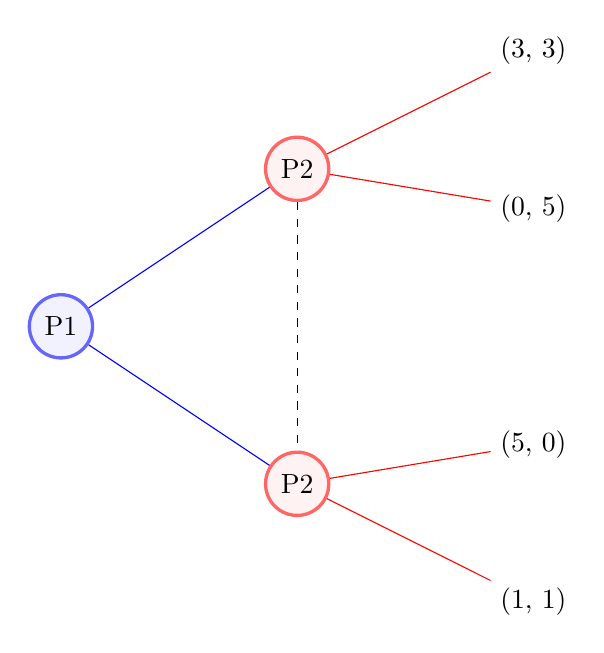
\begin{tikzpicture}
    \node[circle, draw=blue!60, fill=blue!5, very thick, minimum size=7mm] (P1) at (0, 0) {P1};
    \node[circle, draw=red!60, fill=red!5, very thick, minimum size=7mm]  (P21) at (3, 2) {P2};
    \node[circle, draw=red!60, fill=red!5, very thick, minimum size=7mm] (P22) at (3, -2) {P2};
    \draw[blue, thin] (P1) -- (P21);
    \draw[blue, thin] (P1) -- (P22);
    \node (CC) at (6, 3.5) {(3, 3)};
    \node (CD) at (6, 1.5) {(0, 5)};
    \node (DC) at (6, -1.5) {(5, 0)};
    \node (DD) at (6, -3.5) {(1, 1)};
    \draw[red, thin] (P21) -- (CC);
    \draw[red, thin] (P21) -- (CD);
    \draw[red, thin] (P22) -- (DC);
    \draw[red, thin] (P22) -- (DD);
    \draw[black, dashed] (P21) -- (P22);
\end{tikzpicture}
    \caption{The extensive form representation of the PD.}\label{fig:PD_game_tree}
\end{figure}

\begin{definition}
According to~\cite{Webb2007}, a \textit{subgame} is a sub-graph of the game tree
such that:
\begin{itemize}
    \item The sub-graph begins at a decision node, say \(x_{i}\);
    \item This node, \(x_{i}\), is the only element contained in its information
    set; and
    \item The sub-graph contains all of the decision nodes which follow \(x_{i}\).
\end{itemize}   
\end{definition}

This leads to the following definition of \textit{subgame perfect equilibria},
also adapted from~\cite{Webb2007}.

\begin{definition}
    A \textit{subgame perfect equilibrium} is a Nash equilibrium which satisfies
    the condition that the strategies played define a Nash equilibrium in every
    subgame.
\end{definition}

Hence the strategy defined in Theorem~\ref{thm:seq_of_stage_NE} is a subgame
perfect equilibrium. A few final definitions are now highlighted before
introducing the Folk Theorem.

\subsubsection{Final Definitions Needed}\label{subsubsec:Final_Defs_Needed}
Now, in order to be able to discuss the payoffs of strategies in infinite games,
a few final definitions are required.

\begin{definition}
In~\cite{Knight2017b} a \textit{discounted payoff} is defined as:
\begin{equation}
    V_{i}(\sigma) = \sum_{t=1}^{\infty}{\delta^{t-1}U_{i}(\sigma)},
\end{equation}
where the discount factor, \(\delta \), can be thought of as the probability
that the game continues. That is, the probability that another stage game will
be played. 
\end{definition}\label{def:disc_payoff}

Definition~\ref{def:disc_payoff} can be used to define \textit{average payoffs}.

\begin{definition}
    According to~\cite{Knight2017b}, the \textit{average payoffs} per stage
    game, are given by:
   \begin{equation}
        \frac{1}{\overline{T}}V_{i}(\sigma) = (1-\delta)V_{i}(\sigma),    
    \end{equation}
    where \(\overline{T} = \frac{1}{1-\delta}\) is the average length of a game. 
\end{definition}

Finally, Figure~\ref{fig:Feasible_Payoff_Plot} shows those payoffs which are
individually rational for a two player version of PD\@. In
general, an \textit{individually rational payoff} is an average payoff which
exceeds those obtained in the stage Nash equilibria for all
players~\cite{Knight2017b}. Often the Nash equilibrium payoff is not the
optimal payoff players could achieve.

\begin{figure}
    \centering
    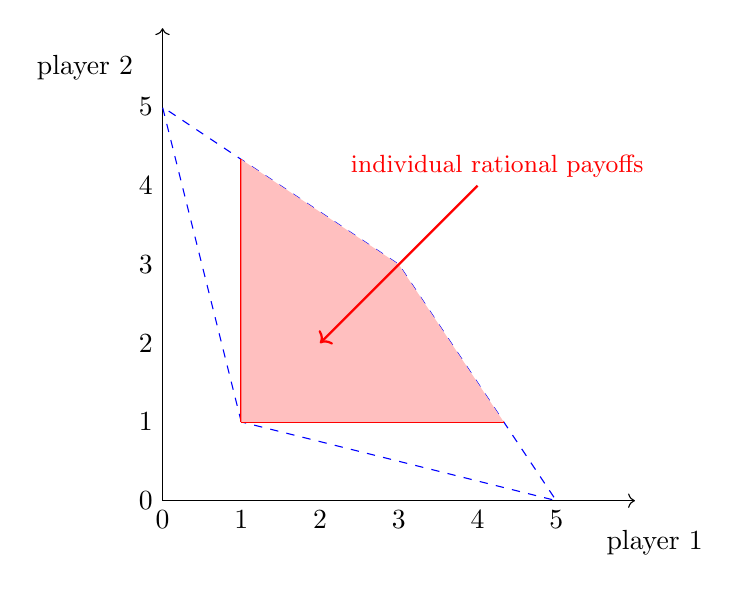
\begin{tikzpicture}
    \draw[->] (0,0) -- (6,0);
    \node[below] at (6.25, -0.25) {player 1};
    \draw[->] (0,0) -- (0,6);
    \node[left] at (-0.25, 5.5) {player 2};
    \foreach \x/\xtext in {0,1,2,3,4,5}
        \node[below] at (\x, 0) {$\xtext$};
    \foreach \y/\ytext in {0,1,2,3,4,5}
        \node[left] at (0, \y) {$\ytext$};
    \draw[blue, dashed] (1,1) -- (0,5) -- (3,3) -- (5,0) -- (1,1);
    \draw[red, thick] (1, 1) -- (1, 13/3);
    \draw[red, thick] (1, 1) -- (13/3, 1);
    \fill[red!25] (1, 1) -- (1, 13/3) -- (3, 3) -- (13/3, 1) -- (1, 1);
    \node[red] at (4.25, 4.25) {\small individual rational payoffs};
    \draw[red, ->, thick] (4, 4) -- (2, 2);
\end{tikzpicture}
    \caption{A plot highlighting the individually rational payoffs for the PD.}\label{fig:Feasible_Payoff_Plot}
\end{figure}

\section{Folk Theorem}\label{sec:Folk_Thm}
This section contains the statement and proof of the main theorem in this project.

According to~\cite{Webb2007}, the Folk Theorems are
so-called because their results were well-known before a formal proof was
provided. In general, these theorems state that players can achieve a better
payoff than the Nash equilibrium (if the Nash equilibrium payoff is not optimal)
when the stage game is repeated many times and the probability of the game
continuing is high enough. 

It is believed that~\cite{friedman1971non} was one of the
first to provide a formal proof to the widely accepted Folk
Theorem~\cite{Abreu1994, Webb2007}. Thus, the presentation of the statement and
proof given here is adapted from~\cite{friedman1971non} as well as~\cite{Knight2017b}.

\begin{theorem}
    Assume the conditions provided in Section~\ref{subsec:Assumptions} are
    satisfied for the given infinite repeated game. Then, for any individually
    rational payoff \(V_{i}\), there exists a discount parameter \(\delta^{*}\)
    such that for all \(\delta_{i}\), \(0 < \delta^{*} < \delta_{i} < 1\) there
    is a subgame perfect Nash equilibria with payoffs equal to \(V_{i}\).
\end{theorem}\label{thm:Folk}

\subsection{Assumptions}\label{subsec:Assumptions}
Here, the assumptions which Friedman~\cite{friedman1971non} requires the
infinite repeated game to satisfy in order for Theorem~\ref{thm:Folk} to hold are listed.
\begin{enumerate}
    \item The mixed action sets, \(\Sigma_{i}\) are compact and convex for all
    \(i\in N\). 

    \item The payoff functions, \(U_{i}: \Sigma \to \mathbb{R}\), are continuous
    and bounded for all \(i\in N\).

    \item The \(U_{i}(\sigma)\)s are quasi-concave\footnote{According
    to~\cite{Stover}, a real-valued function \(f\), defined on a convex subset
    \(C \subset \mathbb{R}^n\), is \textit{quasi-concave} if for all \(\alpha
    \in \mathbb{R}\), the set \( \{ x \in C : f(x) \ge a \} \) is convex.}
    functions of \(sigma_{i}\) for all \(i\in N\).

    \item If  \(U_{i}^{\prime} \le U_{i}^{\prime\prime}\), for all \(i\in N\)
    and \(U_{i}^{\prime}, U_{i}^{\prime\prime} \in \mathcal{U}\), then, for all
    \(U_{i}^{\prime} \le U \le U_{i}^{\prime\prime}\), \(U \in \mathcal{U}\). Here, \(\mathcal{U}\)
    is defined to be the set of feasible payoffs, \( \{ U(\sigma) : \sigma \in
    \Sigma \} \), where \(U(\sigma) = (U_{1}(\sigma), U_{2}(\sigma), \ldots,
    U_{N}(\sigma))\).

    \item \(\mathcal{U}^{*}\) is concave, where \(\mathcal{U}^{*} \subset \mathcal{U}\) denotes the
    set of all Pareto optimal payoffs\footnote{The paper~\cite{friedman1971non} defines a
    \textit{Pareto optimal payoff} as a point in the payoff space
    \(U_{i}(\sigma^{*})\) which satisfies the conditions: \(\sigma^{*} \in
    \Sigma \) and \(U_{i}(\sigma^{*}) > U_{i}(\sigma)\) for all \(i \in N\)}.

    \item All stage games are identical in the infinitely repeated game.

    \item The discount parameter, \(\delta \), is equal in all time periods.
    
    \item The stage game has a unique Nash equilibrium.

    \item The Nash equilibrium is not Pareto optimal\footnote{That is, the
    payoff yielded from the Nash equilibrium is not a Pareto optimal payoff.}. 
\end{enumerate}

Note~\cite{friedman1971non} later goes on to prove that assumptions
six to nine can be removed with only a small effect on the result. However,
since the game being studied in this project is the IPD (which satisfies
all the above assumptions), this generalisation will be omitted. Only the
proof of the original theorem will be provided.

\subsection{Proof of the Folk Theorem}

\begin{proof}
    Consider the set of all actions which yield greater payoffs than the Nash
    equilibrium, denoted by:
    \begin{equation}
        B = \{\sigma : \sigma \in \Sigma, U_{i}(\sigma) > U_{i}(\sigma^{*}), i \in N\}
    \end{equation}
    where \(\sigma^{*}\) is the Nash equilibrium strategy. Define the following trigger strategy:
    \begin{equation}
        \sigma_{i1} = \sigma_{i}^{\prime};~~~
        \sigma_{it} = \begin{cases}
            \sigma_{i}^{\prime}, & \quad \text{if } \sigma_{j\tau}=\sigma_{j}^{\prime} \ j \ne i, \tau=1, 2, \ldots, t-1, t=2, 3, \ldots \\
            \sigma_{i}^{*}, & \quad \text{otherwise},
        \end{cases}
    \end{equation}\label{eqn:trigger_strategy}
    where \(\sigma_{i}^{\prime} \in B\). In words, the \(i\)th player will choose \(\sigma_{i}^{\prime}\) unless any
    other player does not play \( \sigma_{j}^{\prime}\), in which case they
    continue by playing their Nash equilibrium action, \(\sigma_{i}^{*}\). 
    
    Now, by definition, the strategy in~\eqref{eqn:trigger_strategy} is an
    equilibrium of the repeated game if 
    \begin{equation}
        \sum_{\tau=0}^{\infty}{\delta_{i}^{\tau}U_{i}(\sigma_{i}^{\prime})} > U_{i}(\sigma_{-i}^{\prime}, t_{i}) + \sum_{\tau=1}^{\infty}{\delta_{i}^{\tau}U_{i}(\sigma^{*})},~~~ i \in N,
    \end{equation}
    which can be rearranged to 
    \begin{equation}
        \frac{\delta_{i}}{1-\delta_{i}}[U_{i}(\sigma^{\prime}) - U_{i}(\sigma^{*})] > U_{i}(\sigma_{-i}^{\prime}, t_{i}) - U_{i}(\sigma{\prime}),~~~ i \in N,
    \end{equation}
    where \(U_{i}(\sigma_{-i}^{\prime}, t_{i}) = \max_{\sigma_{i} \in
    \Sigma_{i}}{U_{i}(\sigma_{-i}^{\prime}, \sigma_{i})}\), \(t_{i} \in
    \Sigma_{i}\). Note, \(\sigma_{-i} = (\sigma_{1}, \ldots, \sigma_{i-1},
    \sigma_{i+1}, \ldots, \sigma_{n})\) is the strategy vector with the \(i\)th
    player removed.

    To check if this strategy is indeed a best response to all others players,
    who are executing the same strategy in~\eqref{eqn:trigger_strategy},
    consider their alternatives. The \(i\)th player has two options. Either
    they execute the strategy~\eqref{eqn:trigger_strategy}, or they play the
    strategy in which \(\sigma_{i1} = t_{i}\). The latter implies \(\sigma_{i\tau} =
    \sigma^{*}\) will be the best response as every other player will convert
    to \(\sigma_{j\tau} = \sigma^{*}\), for all \(\tau > 1\). Note that any
    other strategy is weakly dominated by one of these two, since playing
    \(t_{i}\) in any other stage \(\tau \ne 1\) will yield less gains due to increased discounting.

    Now if, from playing the Nash equilibria, the discounted loss 
    \begin{equation}
        \frac{\delta_{i}}{1-\delta_{i}}[U_{i}(\sigma^{\prime}) -
        U_{i}(\sigma^{*})],
    \end{equation}\label{eqn:discounted_loss}
    is greater than the gain achieved by playing
    \(t_{i}\) against \(\sigma_{-i}^{\prime}\), then the rational
    strategy choice for player \(i\), assuming all other players are
    executing~\eqref{eqn:trigger_strategy}, is to play~\eqref{eqn:trigger_strategy}.
    
    Observe, as the discount parameter, \(\delta \to 1\) from
    below, the discounted loss in~\eqref{eqn:discounted_loss} tends to infinity.
    However, the gain obtained from playing \(t_{i}\), that is,
    \(U_{i}(\sigma_{-i}^{\prime}, t_{i}) - U_{i}(\sigma{\prime})\) is finite.
    Thus, for all \(\sigma_{i}^{\prime} \in B\) there exists a \(\delta^{*} \in
    (0, 1)\) such that for all \(\delta_{i} > \delta^{*}\), the
    strategy~\eqref{eqn:trigger_strategy} is optimal against the same strategy
    for all players \(j \ne i\). Therefore, if the conditions are true for all
    players \(i = 1,2,\ldots,n\), the strategy \((\bar{\sigma}_{1},
    \bar{\sigma}_{2}, \ldots, \bar{\sigma}_{n})\), where  \(\bar{\sigma}_{i}\)
    denotes~\eqref{eqn:trigger_strategy}, yields a Nash equilibrium.

    Finally, by construction, the strategy~\eqref{eqn:trigger_strategy} is
    indeed a subgame perfect equilibrium. 
\end{proof}


\section{Aims of the Project}\label{sec:Aims_of_the_Project}
This project stemmed from an initial idea presented in a game theory assignment
completed by the author. The topic of this coursework was Nash equilibria of
repeated games and the two graphs, as presented in Figure~\ref{fig:CW_plots}, were
obtained.

\begin{figure}
    \centering
        \begin{subfigure}{0.45\textwidth}
            \centering
            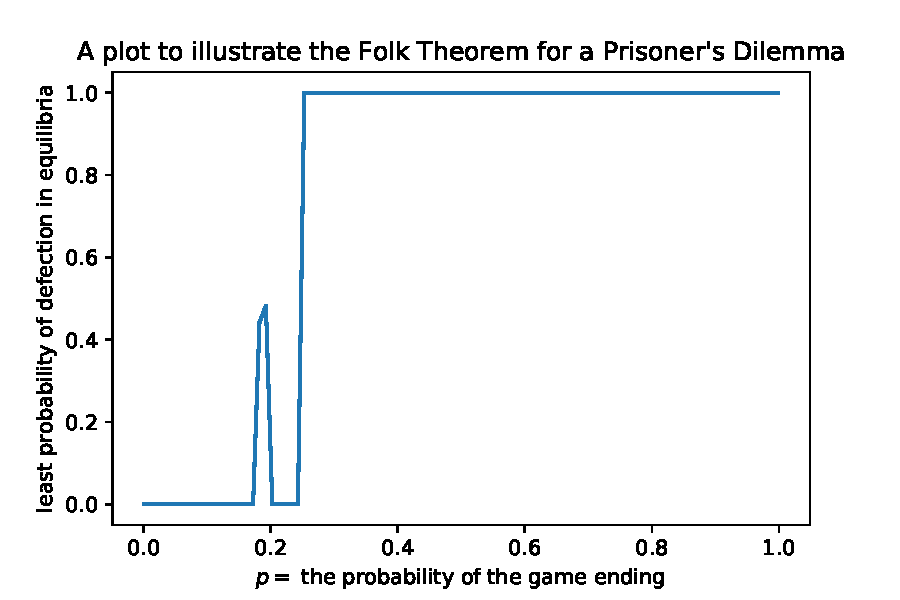
\includegraphics[width=\textwidth]{CW-graph-1.pdf}
            \caption{A plot of the least probabilities of defection against the strategies: \textit{Cooperator}, \textit{TitForTat} and \textit{Random}. Here, the \(p\)-threshold is approximately 0.25.}\label{fig:CW_graph_1}
        \end{subfigure}
        \hspace{3pt}
        \begin{subfigure}{0.45\textwidth}
            \centering
            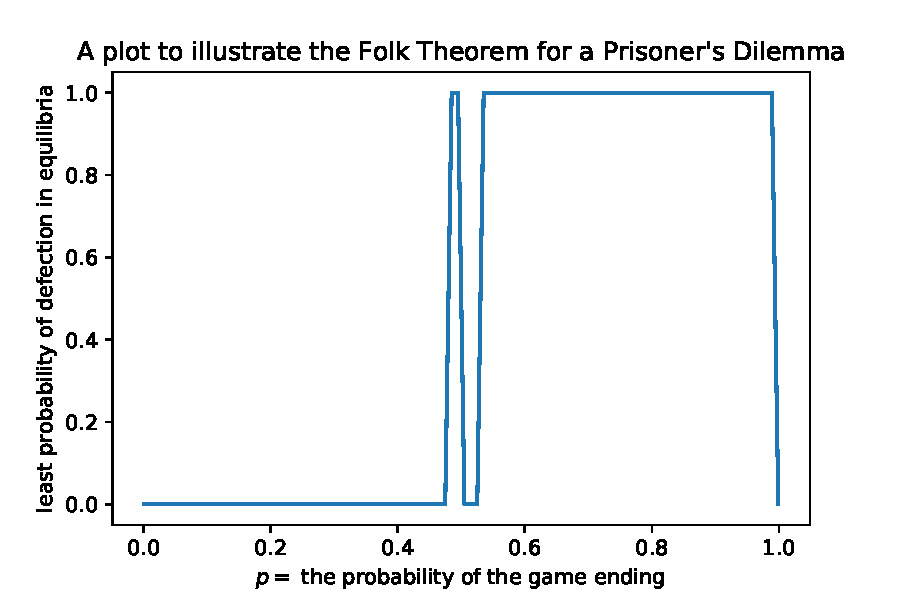
\includegraphics[width=\textwidth]{CW-graph-2.pdf}
            \caption{A plot of the least probabilities of defection against the strategies: \textit{Winner21}, \textit{AntiTitForTat} and \textit{OmegaTFT}. Here, the \(p\)-threshold is around 0.5.}\label{fig:CW_graph_2}
        \end{subfigure}
        \caption{Original plots obtained which influenced the subject of this project.}\label{fig:CW_plots}
\end{figure}

Figure~\ref{fig:CW_plots} was obtained from repeating IPD tournaments which are
implemented in Python via the package Axelrod~\cite{axelrodproject}. In general,
these tournaments are a group of strategies, who all compete in a variety of
round-robin, two-player IPDs with the aim of achieving the largest payoffs. The
implementation in Axelrod allows for the simulation and analysis of IPD
tournaments under different environments. For example:
\begin{itemize}
    \item It is possible to vary the number of strategies making the groups competing in the
    tournament\footnote{In this project, the group of strategies will be
    referred to as a \textit{player set} for clarity.
    Consider Figure~\ref{fig:CW_graph_1}, the player set here consists of the
    strategies: \textit{Cooperator}, \textit{TitForTat}, \textit{Random} and
    \textit{Defector}.}.
    
    \item Both finite and infinite IPD can be considered. The infinite IPD is
    simulated through the scenario of a probabilistic ending, denoted throughout
    this study as \(p_{e}\)\footnote{The probability of the game ending,
    \(p_{e}\), will also be referred to as a game-ending
    probability, in this project.}. Note, \(p_{e}\) is related to the discount
    parameter, \(\delta \), introduced in Definition~\ref{def:disc_payoff}, by \(p_{e}
    = 1 - \delta \).
    
    \item Varying levels of noise can be introduced. This is referred to as
    \textit{standard PD noise}\footnote{Note, there are three potential sources
    of noise within an IPD tournament. In order to differentiate between them
    the following terms are used. \textit{Standard PD noise} to refer to the
    probability of an action being altered; \textit{stochastic player noise} to
    refer to the noise induced by a stochastic strategy; and \textit{unexpected
    noise} to refer to noise which is expected from running numerical experiments.} within this report. According
    to~\cite{glynatsi2020meta}, \textit{standard PD noise} is the probability,
    \(p_{n}\), of an action being altered within any particular round. That is,
    the probability of a \(C\) being seen as a \(D\) and vice versa.
\end{itemize}

The two plots seen in Figure~\ref{fig:CW_plots} were yielded from setting \(p_{n} =
0\), the player set size equal to four, \(p_{e}\) taking 100 distinct values
within (0, 1) and each tournament to repeat 100 times. The graphs show the least
probability of defection obtained in the Nash equilibria of the corresponding
game. Note, the `corresponding game' here refers to the matrix of mean payoff
values which can be calculated from the tournament results of each strategy
(see Chapter~\ref{ch:Methods} for further explanation of this).  

From Figure~\ref{fig:CW_plots}, it can be seen that there is a clear game-ending
probability \(p_{e}\) for which the least probability of defection goes to zero.
In this project, this probability is defined as a \textit{\(p\)-threshold}.
However, what was most intriguing was that the two different games obtained had
a different \(p\)-threshold. This is approximately 0.25
for Figure~\ref{fig:CW_graph_1} but for Figure~\ref{fig:CW_graph_2} the threshold
appears at around 0.5. This initiated the idea to investigate whether there are
any specific characteristics of an IPD tournament that affect the value of the
\(p\)-threshold.

Therefore, the aims of this project are as follows:
\begin{enumerate}
\item To provide a review of past and present literature already published in
the field of folk theorems;

\item To develop a program which executes a large experiment involving
tournaments of the IPD with differing environments to obtain
graphs similar to those in Figure~\ref{fig:CW_plots}; and

\item To perform analyses on where the \(p\)-thresholds seem to lie and
whether it is affected by the change in the number of players, levels of
standard PD noise, etc.
\end{enumerate}

\chapter{Literature Review}\label{ch:Lit_Review}

The folk theorems are a class of results which generally state that for repeated
games, any feasible and individually rational payoff vector can be achieved as a
subgame perfect equilibrium if the players are patient enough~\cite{Li2019}. The
origin of these theorems is unknown however written proof and
research involving these ideas first appeared
in~\cite{aumann1976long,Friedman1971,Rubinstein1979} in the 1970s. Since then,
many generalisations and refinements of
the ideas have been explored, for different games, including:
games with private monitoring~\cite{Hoerner2006,Matsushima2004, Peski2012}, sequential
games~\cite{Bhaskar1998,Gossner1996,Wen2002} and games of complete
information~\cite{Abreu1994,Benoit_1985,Bernergard2019}, to
name a few. Due to the identification of further equilibria (as compared with
the stage game), which are key in predicting future behaviour, these theorems
have been commented on as `fundamental' in the theory of non-cooperative
games by~\cite{Hoerner2006, Li2015}. On the other hand, the majority of the strategies used in the
proofs assume the identification of individual deviators~\cite{Masso1989} which may not
be realistic in certain situations. Hence, an area of research on the so-called
`anti-folk theorems' was introduced~\cite{Masso1989,Peski2012,Yoon2001}. Folk theorems appear to still be an
active area of research today~\cite{Ikeda2020, Parras2020, Wang2020} with many differing applications.
Therefore, in this chapter, a review of the literature on this topic is provided
with papers ranging from the `original' ideas in the 1970s to applications of
the theorems in 2020. 


\section{First Papers}\label{sec:First_Papers}
According to~\cite{Abreu1994}, the earliest work on Folk-type theorems is~\cite{Friedman1971}. In~\cite{Friedman1971}, infinitely repeated games with
discounting are considered. In particular, focus is on a class of strategies,
now known as \emph{grim trigger}. These are used to prove that, for any feasible
and individually rational payoff vector, there exists a discount parameter such
that a subgame perfect equilibrium with payoffs equal to that vector exist. This
is first shown under the constraints of: identical stage games, constant
discount parameter and unique Nash equilibrium that is not Pareto optimal. This
is in addition to those made on the strategy and payoff spaces. However, a more
general result is then given which removes these restrictive conditions.
The application of oligopoly is used throughout~\cite{Friedman1971}. Moreover,
he introduces the notion of `temptation'. He motivates this through the
explanation that `threat' is no longer ``credible'' since players are unable to
communicate in non-cooperative games. On the other hand, `temptation' is said to be analogous to `threat'.

In contrast to this,~\cite{aumann1976long} presents folk theorems for infinite
games without discounting, assuming payoffs take a ``limiting average form''.
This choice is justified through the statement that, as the discount rate
approaches zero, the limit of the discounted sum behaves similarly to the
limiting average payoff
form. However, trigger strategies are still required in the proof and, for
simplicity, two player games are assumed. Two folk theorems are
proven in this paper with the latter one discussing subgame perfect equilibria
similar to~\cite{Friedman1971}, whilst the former is a more generic version of
the theorem. In~\cite{aumann1976long} it is discussed that, though the generic version of
the theorem does exist, the subgame perfect equilibrium points allow for more
`believable' behaviour. They conclude by considering an example in which payoffs
are discounted. A similar approach is taken in~\cite{Rubinstein1979}, with the
statement of a folk theorem for infinite games with no discounting and the
existence of subgame perfect equilibria. The only difference being the use of an
``overtaking criterion'' instead of a ``limit of the mean
criterion'' as in~\cite{aumann1976long}.


\section{Games with Complete Information}\label{sec:Games_with_Complete_Information}
Folk theorems of games assuming complete information are studied
in~\cite{Abreu1994, Bernergard2019}. That is, all players have common knowledge
of payoff functions and strategies. Paper~\cite{Abreu1994} focuses on the
necessary and sufficient conditions required for a folk theorem proof. They
state that feasibility and individual rationality of the payoff vector are
necessary, and also approximately sufficient, conditions for a payoff to be in
the equilibrium. This is followed by a discussion on the full dimensionality
constraint first introduced by~\cite{Fudenberg1986} and often used in proving
folk theorems. It is highlighted in~\cite{Abreu1994} that the equality between
the dimension of the convex hull of feasible payoffs and the number
of players is a sufficient condition. This provides motivation for the main result of the paper; the
introduction of a `non equivalent utilities' condition, which is proved to be
sufficient and almost necessary for a folk theorem. The condition, as indicated
here, is weaker than the aforementioned full dimensionality condition. According
to~\cite{Abreu1994}, it only requires ``no pair of players have equivalent utility functions''.

Similarly, a folk theorem for complete information
games with subgame perfect equilibria is proved in~\cite{Bernergard2019}. However, instead of exponential
discounting as in~\cite{Abreu1994, Fudenberg1986}, he assumes discounting is
present-biased. That is, the discount function implies a player is more willing
to alter an event in the future than altering a current event. The folk theorem
is proved in cases of where the player is time consistent (prefers to maximise
their initial preferences) and time inconsistent (prefers to maximise current
preferences). In~\cite{Bernergard2019}, the notion of `patience' is taken to be the sum of all discount
factors. Also considering time consistent and inconsistent
players~\cite{Li2019}, discusses folk theorems with respect to time-dependent
discounting. In contrast
to~\cite{Bernergard2019}, the long-term characterisation of `patience' is taken
as the discount factors at all stages uniformly converge to one. Motivation for
the study of time-dependent discounting is explained by empirical studies which
seem to suggest that a player's time is unstationary, rather than stationary
which is assumed in most discounted game models.


\section{Games with (Imperfect) Private Monitoring}\label{sec:Games_with_(Imperfect)_Private_Monitoring}
In the late 1990s attention turned to games with imperfect monitoring. That is,
a player's actions can no longer be observed accurately, instead public or
private signals are detected~\cite{Durlauf2016}. According to~\cite{Matsushima2004}, games with (imperfect) public
monitoring were the first to be considered. More recent
studies in this area include~\cite{Chassang2011,Kandori2006}.
Repeated games with public monitoring are stated
in~\cite{Kandori2006} to give a
suitable model for studying long term relationships. They say intuition
suggests that cooperation becomes easier to sustain as action observability
improves. However,~\cite{Kandori2006} continues to show that this intuition is
false, by considering a repeated public monitored game which satisfies ``the
limit perfect public equilibrium payoff set can achieve full efficiency
asymptotically as public information becomes less sensitive to hidden actions''.
They give an example which violates the sufficient condition given
in~\cite{Maskin1994} yet a folk theorem can still be obtained. This paper mainly
focuses on
the PD but, similarly to~\cite{Abreu1994}, they state an example
which satisfies the folk theorem without the full dimensionality condition. 

The notion of a robust equilibrium to incomplete
information is considered in~\cite{Chassang2011}. That is, if the equilibrium
yielded is near the original equilibrium for all perturbed games consisting of a
small independent and identically distributed information shock. Conversely to~\cite{Friedman1971},
they discuss the implication of grim trigger strategies not being robust when
the aim is to sustain cooperation. A folk theorem is proved in robust equilibria
for games of public monitoring, however~\cite{Chassang2011} highlights that a
much stronger condition is needed in comparison to the full dimensionality
requirement in~\cite{Maskin1994}.

As of 2004, according to~\cite{Matsushima2004}, repeated games with private
monitoring was a relatively new area of study. In this paper, conditional
independence of signals
is assumed in order to show a folk theorem for the IPD\@. Applications to
duopolies are then described. Another study to consider a folk theorem for the
IPD is~\cite{Ely2002}. Using a similar definition of robustness
to~\cite{Chassang2011},~\cite{Ely2002} proves that for a discounted PD with private monitoring technologies, a folk theorem with robust
equilibrium strategies can be obtained. In particular, they consider
almost-perfect private monitoring and a limit folk theorem (for sequential
equilibria) follows. In a similar paper,~\cite{Ely2005} introduce the idea of
``belief-free'' equilibrium strategies; a property which implies the belief of
an opponent's history is not required when obtaining a best response. They use
these strategies in proving a folk theorem for the two-player PD
however, for general games, the set of belief-free payoffs is not large enough
to provide a folk theorem. Moreover,~\cite{Ely2005} highlight that, for a larger
number of players, the calculation of the payoff set becomes significantly
harder.

In contrast to this,~\cite{Hoerner2006} discusses a folk theorem using
strategies that, although are not belief-free, still make beliefs ``irrelevant''
at the start of each T-block of stage games. Their result is much more generic
than~\cite{Ely2005} since it applies to N-player finite games under the
assumption of full dimensionality with private, but almost-perfect, monitoring.
The T-block strategies mentioned above are modified in~\cite{Yamamoto2009,Yamamoto2012} such that they ``can support any vector in the belief-free
equilibrium payoff set''. This modification results in belief-free equilibrium
strategies. The results in~\cite{Yamamoto2009,Yamamoto2012} are generalisations
from the two-player PD in~\cite{Ely2005} to the corresponding
N-player game.


\section{Games with Communication}\label{sec:Games_with_Communication} 
Academics introduced games with communication to deal with the complications
faced with imperfect monitoring. For example, according to~\cite{Kandori2003},
games with public monitoring can obtain a folk theorem under weaker assumptions
than those given in~\cite{Maskin1994}, if communication is introduced.
In this paper, communication is a message, taken from the set of possible
actions, which the players give simultaneously after choosing an action and
observing a signal. He proves a folk theorem for symmetric games
with four or more players, without the assumption of the number of signals
relevant to the number of actions.

Regarding private monitoring,~\cite{Obara2009} claims repeated games are ``very
difficult to analyse without communication''. Thus examples of papers, proving
folk theorems for these games with communication,
include~\cite{Fudenberg2008,Li2010,Obara2009}. A
`Nash threats' folk theorem is proved in~\cite{Fudenberg2008},
similar to~\cite{Friedman1971}, in the case of almost public information games,
without independent signals, for two players. In this paper, communication is
defined in the form of announcements where each set of announcements is the same
for all players. The decision to only consider two player games is justified
in~\cite{Fudenberg2008} by
highlighting that, although the results can be generalised, in certain cases it
can be seen as advantageous to have additional players. Similarly,~\cite{Obara2009} proves a `Nash threats' folk theorem for private monitoring games
with communication. He increases the number of environments where the folk
theorem is applicable through developing further the idea of ``delayed
communication'', as given in~\cite{Compte1998}. In addition,~\cite{Obara2009}
uses the assumptions of correlated private signals; and each player's deviation
from strategy is statistically identifiable from the other players' signals. A model of private monitoring and communication
within games is also considered in~\cite{Li2010}. He has the aim of increasing the number of applicable
environments for~\cite{Kandori1998} frequent
communication folk theorem. The paper states that~\cite{Kandori1998} assumed only private signals were publicised in this theorem
but if other information was useful and communication was free and legal then
players would also want to share their actions. This motivates the reasoning
behind the paper. However, assumptions of full dimensionality, and the
number of actions and signals, are still required. 

Another paper which considers communication is~\cite{Block2016}, regarding self
referential games with codes of conduct. These codes are descriptions of how the
players and opponents should play and an application to computer algorithms is
provided. Two folk theorems are proved: one assuming common knowledge of the
codes of conduct, and the other where only certain players observe certain
codes. The latter is the main result of the paper and is motivated by the fact
that, often, individuals have good knowledge of those closest to them but not
the whole community. Moreover,~\cite{Block2016} obtain the sufficient condition
that, with public communication, if every player is observed by another two
opponents, then a folk theorem is yielded.


\section{Finite Horizon Games}\label{sec:Finite_Horizon_Games}
Another area of interest is the existence of folk theorem-type results for games
of finite repetition. In~\cite{Benoit_1985}, the case of
finitely repeated games of complete information and the associated subgame
perfect equilibria is explored. Despite the existence of games which, when
repeated finitely, ``produce no non-cooperative equilibrium outcomes''; they
state there may be subgame perfect equilibria of finite-repeated games, when the
corresponding single game has multiple equilibria. Indeed, using their ``three
phase punishment'',~\cite{Benoit_1985} prove that ``any rational and feasible
payoff vector can be obtained in the limit''. This is assuming the feasible
payoff region has dimension equal to the number of players and each player has
two Nash equilibrium payoff values. In a similar manner,~\cite{ANGELOVA2011}
considers an alternative version of the PD in which an additional strategy is
included. This gives a second pure-strategy equilibrium and a folk theorem
result for the finitely repeated version of this game. 

Although not strictly a finite game,~\cite{Fujiwara-Greve2018} study a repeated
game in which players may ``strategically terminate'' it. In particular, this
involves the incorporation of a voting-step, at the start of each repetition,
where a certain number of players decide whether or not to keep interacting.
This is motivated by the increasing possibilities of ending business
partnerships due to more technology and knowledge. A general folk theorem for
any stage game (with the additional voting), which is satisfied ``for all
majority rules except the unanimous ending'' is proved by~\cite{Fujiwara-Greve2018}. Indeed, for the unanimous ending rule, they
show that the theorem may not hold but sufficient conditions are
provided for when it is satisfied.


\section{Stochastic and Sequential Games}\label{sec:Stochastic_and_Sequential_Games}
Other game types to have associated folk theorem results include
stochastic~\cite{Dutta1995} and overlapping generation~\cite{Bhaskar1998,
Gossner1996}.

It is explained in~\cite{Dutta1995} that, often, the standard assumption of ``a
completely unchanging environment'', within the theory of repeated games, is not
reliable in applications. This reasoning is the motivation for studying, the
more generic, stochastic games. These games may not have a pre-decided stage
game, instead a `state variable' is used to represent its environment which
alters according to``initial conditions, player's actions, and the transition
law''. The paper~\cite{Dutta1995} discusses equilibrium payoffs in the case of
very patient players, without the
need for the Markovian property. Specifically, perfect monitoring is assumed,
along with asymptotic state independence and either of payoff asymmetry or full
dimensionality. Two folk theorems are proved in~\cite{Dutta1995}: one with
unobservable mixed strategies (in which case, fully dimensionality is required)
and also, similar to~\cite{Abreu1994}, one with the slightly weaker condition of
payoff asymmetry (here, mixed strategies have to be observed).

Both\cite{Bhaskar1998, Gossner1996} provide insight into folk theorems
associated with overlapping generation games. These are similar to the repeated
normal form games except that the players are considered to be finite.
That is, each player is involved in a certain number of stage games before they
are replaced by another, identical player. A variety
of folk theorems are proved in~\cite{Gossner1996} both with and without
discounting and / or observable mixed strategies. He shows that the full
dimensionality assumption is not required in
these games since players are assumed to not end simultaneously. On the other
hand, although~\cite{Bhaskar1998} does provide a folk theorem, his main result
is an anti-folk theorem, see~\autoref{sec:Anti-Folk_Theorems}. He studies games
with imperfect public monitoring and states that, in such overlapping
generational games, cooperation becomes impossible in contrast to repeated
games. Furthermore,~\cite{Bhaskar1998} constructs a mixed strategy equilibrium
folk theorem. However, he goes on to show that these strategies are unstable to
perturbations, resulting in an anti-folk theorem.

A similar study by~\cite{Anderlini2008} looks at dynastic repeated games. These
differ from the overlapping generation games in two aspects: perfect observation
of the past is assumed, and the payoffs obtain no dynastic component. Under the
assumptions of full dimensionality and the existence of a payoff vector which
strictly Pareto dominates the stage game equilibrium,~\cite{Anderlini2008}
proves a folk theorem for private communication games, with greater than three
players, in sequential equilibria.

Considering now sequential games, in which players do not choose their action
simultaneously,~\cite{Wen2002} introduces a concept of effective minimax values
before proving a corresponding folk theorem. In his model, players pick actions
in groups. Thus the effective minimax value is defined to be the lowest
equilibrium payoff a player will receive, even if none of their opponents have
equivalent utilities. According to~\cite{Wen2002}, his folk theorem can be
applied to other game models as it is a ``uniform characterisation''.


\section{Anti-Folk Theorems}\label{sec:Anti-Folk_Theorems}
A common theme in the proofs of folk theorems is the use of strategies which
``identify and punish'' deviators~\cite{Masso1989}. However, as soon as the game
contains incomplete / imperfect information, deviators cannot necessarily be
identified. This yields a much smaller equilibrium set and these results are
termed ``Anti-Folk Theorems''. This description of anti-folk theorems is adapted
from~\cite{Masso1989}, who state the original term was given
in~\cite{Dubey1984,Kaneko1982}. An anti-folk theorem is proved
in~\cite{Masso1989} using the ``long-run average criterion'' instead of the
discounted criterion.

Considering similar models to~\cite{Bhaskar1998, Gossner1996}, an anti-folk theorem for a limited-observability overlapping generations
model is obtained in~\cite{Yoon2001}. They show that cooperation cannot be
sustained when new players can only observe recent history. This is in contrast
to the folk theorems obtained under
the assumption of common knowledge of all past actions. Though the results
in~\cite{Yoon2001} are
restrictive in certain cases, they justify the work by stating it is suitable
for modelling ``high turnover'' rates.

Another game model where an anti-folk theorem has resulted is a repeated game
with private monitoring~\cite{Peski2012}. In this paper the following
three assumptions are made: infinite and connected private monitoring (that is,
infinitely many connected signals); finite past; and independent and identically
distributed shocks affect the payoffs. Under these assumptions,~\cite{Peski2012}
shows the violation of the folk theorem. That is, the equilibria of the repeated
game consist only of the equilibria of the single game.


\section{Evolutionary Stability}\label{sec:Evolutionary_Stability}
Recently, there has been research into the results of the folk theorem with
respect to the evolutionary game theoretic paradigm. Indeed,~\cite{Li2015} state
that the folk theorem is often used to characterise evolutionary stable
strategies. This is since exact solutions using theoretical results from
evolutionary game theory are hard to obtain. However, they show the
assumption that the folk theorem yields all Nash equilibria is misleading. This
is achieved by defining ``type-k equilibria'' which are a refinement of the Nash
equilibria. The set of type-k equilibria is proved
in~\cite{Li2015} to be contained
within the set of repeated-game Nash equilibria using ``reactive strategies''.

In contrast to~\cite{Ely2005,Yamamoto2009,
Yamamoto2012}, who discuss folk theorems using belief-free
strategies,~\cite{Heller2017} discusses the instability in an evolutionary
sense. He shows that the belief-free equilibria are not robust to small
perturbations in games with private monitoring and, in certain cases, this is
extreme. Similar to~\cite{Li2015}, he states that Nash equilibria are used to
predict evolutionary behaviour since they are thought of as stable.
However,~\cite{Heller2017} goes on to show that only the choice of repeated stage-game Nash equilibria satisfy evolutionary stability.  


\section{Recent Applications}\label{sec:Recent_Applications}
In recent years, studies have been applying results of the folk theorem in
various areas, for example, to create algorithms. This section briefly
discusses a few of these.

The folk theorem is used in~\cite{Chowdhary2017} for the creation of a model
which aims to suppress the effects of distributed denial of service attacks.
They claim that all networks suffer from attacks to infrastructure and services. Thus,~\cite{Chowdhary2017}
use the programmability of software defined network environments to perform a
game theoretic analysis. An algorithm is created for reward and
punishment based on the Nash folk theorem. Similarly,~\cite{Wang2020} make use
of the cooperative equilibrium solution from the folk theorem
in~\cite{Friedman1971} to create an algorithm suggested to optimise a
`multi-period production planning based real-time scheduling method', for a job
shop. Also,~\cite{Wang2018} uses the result of the folk theorem in the IPD to
study the cooperation rates of varying agent strategies in a multi-agent system.

Another application of the folk theorem is an algorithm used to obtain
equilibria of a discounted repeated game~\cite{Parras2020}. A new algorithm,
entitled ``Communicate \& Agree'', is introduced in~\cite{Parras2020} to
find equilibria in incomplete information, but perfect monitoring, games. Using
the folk theorem in the algorithm enables the payoffs obtained to be potentially
higher than those achieved by repeating the Nash equilibria of the single game.
However,~\cite{Parras2020} go on to highlight that the algorithm is not always
guaranteed to find equilibria. They say it is dependent on: the discount
factor, sampling density, and whether it is a zero-sum game or not.
Finally, in a different area,~\cite{Ikeda2020} discuss the potential of using
game theoretic ideas in quantum optimal transport. In particular, he defines
the Quantum PD and explores the possibility of a quantum folk
theorem in relation to the corresponding repeated game.


\section{Conclusion}\label{sec:Conclusion}
In this section, an overview into research regarding the folk theorem has been
provided. The research history of the folk theorem spans from the 1970s until
now, with many different models being considered. Examples include: games with
complete information, games with imperfect private monitoring and finite-horizon
games. However, there have also been studies into situations where the folk
theorem does not hold, or the equilibrium strategies used in proving the
theorems are unstable and / or not robust. 
\chapter{Methodology and Experiment Setup}\label{ch:Methods}
In this chapter the methods used to collect the data is provided along with
justifications. This study required the execution of several IPD tournaments and
thus appropriate software needed to be implemented and tested for accuracy. All
the appropriate code, written for this project, is made available in the GitHub
repository (https://github.com/shapperzsm/final-project).

\section{Data Collection Algorithm}\label{sec:Data_Collection_Algorithm}
This section describes the overall algorithm used to obtain the data and the
attributes collected. Firstly, the aim of this exercise was
to illustrate the Folk Theorem and analyse the \(p\)-thresholds via a large
experiment. It was expected that plots similar to Figure~\ref{fig:flk_thm_plt}
would be yielded. This clearly shows that there eventually exists a
\(p_{e}\) where defection is not a rational decision.

\begin{figure}
    \centering
    % Example plot
\begin{tikzpicture}
    \draw[->] (0,0) -- (5.5,0) node[right]{$p_{e}$};
    \draw[->] (0,0) -- (0,5.5) node[above]{$min{\{p_{d}\}}$};
    \draw[red, very thick] (0,0) -- (2,0);
    \draw[red, very thick] (2,0) -- (2,5);
    \draw[red, very thick] (2,5) -- (5, 5);
    \draw[blue, dashed, very thick] (2,-0.5) -- (2,5.5);
    \node[blue] at (4, 3) {$p$-threshold};
    \node[below] at (0,0) {0};
    \node[below] at (5,0) {1};
    \node[left] at (0,5) {1};
    \draw[->, thin] (3.5, 2.75) -- (2.25,0.25);
\end{tikzpicture}
    \caption{An example plot illustrating the \(p\)-threshold as indicated by the Folk Theorem. The minimum probability of defection in equilibria is denoted \(\min \{p_{d}\} \).}\label{fig:flk_thm_plt}
\end{figure}

Therefore, to observe whether any environmental settings of the
tournament do affect the p-threshold, a large amount of data was needed. This
was in order for any observations made to be statistically significant. Figure~\ref{fig:alg_diag} shows
a pictorial representation of the collection method used. Each step visible is
explained in detail throughout this chapter with further references to
appropriate sections.

\begin{figure}
    \centering
    \resizebox{\textwidth}{!}{% Algorithm Diagram
\begin{tikzpicture}[roundnode/.style={circle, draw=green!60, fill=green!5, very
thick, minimum size=7mm}, squarenode/.style={rectangle, draw=red!60, fill=red!5,
very thick, minimum size=5mm},
]
    \node[squarenode](start) {START};
    \node[roundnode](database) [right=of start] {\begin{tikzpicture}
    \draw[thin] (0,2) rectangle (3,4);
    \draw[thin] (0, 2.5) -- (3, 2.5);
    \draw[thin] (0, 3) -- (3, 3);
    \draw[thin] (0, 3.5) -- (3, 3.5);
    \draw[thin] (1, 2) -- (1, 4);
    \draw[thin] (2, 2) -- (2, 4);
    \node at (0.05, 4.25) {\footnotesize create database};
\end{tikzpicture}
};
    \node[squarenode](while) [right=of database] {WHILE NOT STOPPED};
    \node[roundnode](defector) [below=of database] {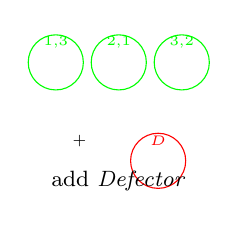
\begin{tikzpicture}
    \draw[green] (0.2, -1) circle (0.35);
    \node[green] at (0.2, -0.75) {\tiny 1,3};
    \draw[green] (1, -1) circle (0.35);
    \node[green] at (1, -0.75) {\tiny 2,1};
    \draw[green] (1.8, -1) circle (0.35);
    \node[green] at (1.8, -0.75) {\tiny 3,2};
    \node at (0.5, -2) {\tiny +};
    \draw[red] (1.5, -2.25) circle (0.35);
    \node[red] at (1.5, -2) {\tiny \(D\)};
    \node at (1, -2.5) {\footnotesize add \textit{Defector}};
\end{tikzpicture}};
    \node[roundnode](select_strat) [right=of defector] {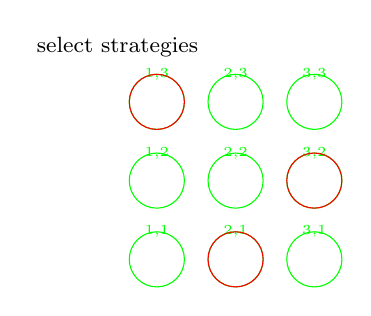
\begin{tikzpicture}
    %\draw[thin, dashed] (0, 0) rectangle (3, 3);
    \foreach \x in {1, 2, 3}
        \foreach \y in {1, 2, 3}
            {\draw[green] (\x-0.5, \y-0.5) circle (0.35);
            \node[green] at (\x-0.5, \y-0.15) {\tiny \x,\y};}
    \node at (0, 3.2) {\footnotesize select strategies};
    \draw[red] (1-0.5, 3-0.5) circle (0.35);
    \draw[red] (2-0.5, 1-0.5) circle (0.35);
    \draw[red] (3-0.5, 2-0.5) circle (0.35);
\end{tikzpicture}};
   \node[squarenode](noise&probs) [left=of defector] {FOR ALL $p_{n}$ \& $p_{e}$};
   \node[roundnode](payoffs) [below=of defector] {\begin{tikzpicture}
    \node at (-0.5, 0) {\tiny payoffs};
    \draw[->, thick] (0.5, 0) -- (0.75, 0);
    \draw[blue, dashed] (0.75, -0.25) rectangle (1, 0.25);
    \draw[blue] (1, -0.5) rectangle (2, 0.5);
    \draw[blue, dashed] (2, -0.25) rectangle (2.25, 0.25);
    \draw[->, thick] (2.25, 0) -- (2.5, 0);
    \node at (3.5, 0) {\tiny Nash eq.};
    \node at (0, 2) {\footnotesize calculating Nash eq.};
    %\node[above] at (1.75, -0.25) {\tiny support enumeration algorithm};
\end{tikzpicture}};
   \node[roundnode](tournament) [left=of payoffs] {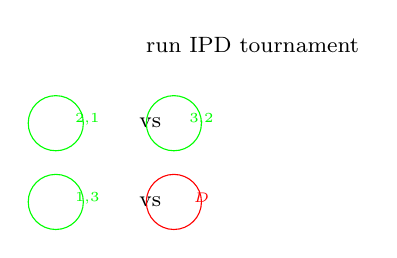
\begin{tikzpicture}
    \draw[green] (0,0) circle (0.35);
    \node[green] at (0.4, 0.05) {\tiny 2,1};
    \node[thick] at (1.2, 0) {\footnotesize vs};
    \draw[green] (1.5, 0) circle (0.35);
    \node[green] at (1.85, 0.05) {\tiny 3,2};
    \draw[green] (0, -1) circle (0.35);
    \node[green] at (0.4, -0.95) {\tiny 1,3};
    \node[thick] at (1.2, -1) {\footnotesize vs};
    \draw[red] (1.5, -1) circle (0.35);
    \node[red] at (1.85, -0.95) {\tiny \(D\)};
    \node at (2.5, 1) {\footnotesize run IPD tournament};
\end{tikzpicture}};
   \node[squarenode](writing) [right=of payoffs] {WRITE RESULTS TO DATABASE};
   \draw[->] (start.east) -- (database.west);
   \draw[->] (database.east) -- (while.west);
   \draw[->] (while.east) -- (15, 0) |- (select_strat.east);
   \draw[->] (select_strat.west) -- (defector.east);
   \draw[->] (defector.west) -- (noise&probs.east);
   \draw[->] (noise&probs.west) -- (-6, -6.12) |- (tournament.west);
   \draw[->] (tournament.east) -- (payoffs.west);
   \draw[->] (payoffs.east) -- (writing.west);
   \draw[->] (writing.east) -- (16, -13.1) |- (select_strat.east);
\end{tikzpicture}
}
    \caption{Representation of the algorithm used to collect the data.}\label{fig:alg_diag}
\end{figure}

From Figure~\ref{fig:alg_diag}, it can be seen that the first step was to set up an
empty database ready to input each tournament result into. 
The specific details of implementation into the algorithm is discussed in Section~\ref{sec:Databases}. However, the choices made on the attributes to
collect are described here. 

\begin{table}
\centering
\begin{tabular}{>{\raggedright}p{0.3\linewidth}>{\raggedright\arraybackslash}p{0.6\linewidth}}
    \toprule
    \textbf{Attribute}                   & \textbf{Description} \\
    \midrule
    experiment\_number           & A unique seed for each tournament run. \\
       
    number\_of\_players           & The number of strategies including the
    Defector. \\
             
    tournament\_player\_set       & A unique number for a particular set of
    strategies. \\
        
    player\_strategy\_name        & The strategy name as given
    in~\cite{axelrodproject}. \\
      
    is\_long\_run\_time            & Characteristic from~\cite{axelrodproject}.
    \\
          
    is\_stochastic               & Characteristic from~\cite{axelrodproject}. \\ 
       
    memory\_depth\_of\_strategy    & Characteristic from~\cite{axelrodproject}.
    \\
       
    prob\_of\_game\_ending         & The value of \(p_{e}\). \\
         
    payoff\_matrix               & A string of the matrix of mean payoff values
    from the tournament. \\
    
    num\_of\_repetitions          & A value indicating how many iterations of
    the tournament is required. \\  
          
    num\_of\_equilibria           & The number of equilibria yielded as output
    from the algorithm. \\
        
    nash\_equilibria             & A string containing the list of equilibria. \\
    
    least\_prob\_of\_defection     & The lowest probability of playing the
    \textit{Defector} obtained from the Nash equilibria. \\ 
     
    greatest\_prob\_of\_defection  & The highest probability of playing the
    \textit{Defector} obtained from the Nash equilibria. \\
    
    noise                       & Level of standard PD noise, \(p_{n}\). \\
                      
    warning\_message             & This column contained a string if the
    algorithm detected potential degeneracy. \\
    \bottomrule
\end{tabular}
\caption{Table of attributes collected.}\label{tab:attr_tab} 
\end{table}

\newpage
Table~\ref{tab:attr_tab}, shows each attribute chosen to be observed in this
study. The attributes experiment\_number and tournament\_player\_set were used
to provide a unique identification for each tournament and set of strategies.
This was to ensure clear separation during analysis. The three characteristics of the strategies
were collected with the aim of analysing the different strategies'
effect on the \(p\)-threshold. The attributes least\_prob\_of\_defection,
warning\_message, number\_of\_players and noise were the most important
attributes to this study. These were the main effects analysed with regards to the \(p\)-threshold and key descriptors of the game. The rest of the attributes
were retained: for evaluation of degeneracy; in order to replicate the
tournaments for validity; and for further research.

Following this came the choice of opponents. The number of opponents selected
ranged from one to eight and were randomly selected from the appropriate
collection of strategies in the Axelrod library~\cite{axelrodproject}. Out of
the 235 strategies currently implemented in Axelrod, only 216 were valid for
this experiment. Since this prroject was considering the Folk Theorem for the IPD,
research strategies which `cheated' (that is, those which return False when
entered into the `obey\_axelrod' function) were omitted. The \textit{Defector} strategy
was also removed as it would later be added to all sets of players. Furthermore,
due to time constraints, the 18 strategies which are classified as having a long
execution time were omitted. 

The actual IPD tournament was run using the original Axelrod tournament
setup~\cite{adeoye2012application} as implemented in the
Axelrod library~\cite{axelrodproject}. This is a round-robin type tournament where each
strategy plays every other strategy once~\cite{axelrod1980effective}.
Each round robin was repeated 500 times to obtain `smoother' estimates of
the mean payoff values. Moreover, each strategy set was run in a tournament for
100 values of \(p_{e}\) within the range \([0.001, 0.999]\). Note, zero was
not included as this implies the tournament would never end and one was
omitted as the tournament would immediately end after the first turn. However,
it is possible for the probabilities within the range \([0.999, 1]\) to be
included in this range; and this is recommended for
future research. These tournaments were also repeated for values of \(p_{n}\) in the set, \( \{0.1, 0.2, \ldots, 1\} \). The main output of interest
from each tournament is the payoff matrix, which is then implemented as the game
matrix in the Nashpy library~\cite{Nashpy2019}.
According to~\cite{axelrodproject}, each entry \(a_{i,j}\) gives the mean payoff
of player \(i\) against player \(j\). Consider the following example:
\begin{equation}
    \begin{pmatrix}
        2.990 &   2.996  &   0.487\\  
        2.996 &   3.000  &   0.989\\
        3.053 &   1.042  &   1.000        
    \end{pmatrix}
\end{equation}\label{eqn:payoff_matrix_ex}
The matrix in~\eqref{eqn:payoff_matrix_ex} is yielded from a three player
tournament with \(p_{e}=0.001 \text{ and } p_{n}=0\). The strategies in this case were \textit{Colbert}; \textit{Tideman and Chieruzzi} and
\textit{Defector}. In this case, the entry \(a_{1,2} = 2.996\) is interpreted as the
mean payoff between \textit{Colbert} and \textit{Tideman and Chieruzzi}. 

For the calculation of the Nash equilibria, the support enumeration
algorithm was used. This algorithm as well as the justification of its use is
provided in Section~\ref{sec:Calculating_Nash_Equilibria}.

Finally, the values obtained were written to the database file. One record is
inserted for each strategy in order to retain all characteristics. Here, any
entries that were not integers or floats had to be converted to strings, in order
to be stored. For example, the payoff matrix given
in~\eqref{eqn:payoff_matrix_ex} is a list and hence could not be inserted into the
database in its current format.


In summary, pseudo code for the overall algorithm is provided
in Algorithm~\ref{alg:folk_thm_explore}.

\IncMargin{2em}
\begin{algorithm}[H]
    \footnotesize
    \DontPrintSemicolon
    \SetKwInOut{Input}{input}
    \SetKwInOut{Output}{output}

    \Input{maximum number of opponents, number of strategy sets for each number
    of opponents, set of \(p_{n}\), set of \(p_{e}\), number of tournament repetitions, the
    database file path, and whether or not support
    enumeration should be used to calculate the Nash equilibria.}
    \Output{a database containing the results as detailed previously.}
    \While{True}{
        \For{each number of opponents}{
            \For{each repetition with the same number of strategies}{
                Randomly select a set of opponents and add in the \textit{Defector}.\\
                \For{each \(p_{n}\)}{
                    \For{each \(p_{e}\)}{
                        Run the IPD tournament.\\
                        Obtain the Nash equilibria and the corresponding
                        probabilities of defection, using the algorithm
                        indicated.\\
                        \For{each player in the current set}{
                            Write the required information to a record in the
                            database file.\\
                        }
                    }
                } 
            }
            Repeat
        }
    }
    \caption{Folk Theorem Exploration}\label{alg:folk_thm_explore}
\end{algorithm}
\DecMargin{2em}

\section{Databases}\label{sec:Databases}
There are many different options regarding types of file available for storage of
data. For example, csv, json, tex, txt, db extensions. These are generally split into
two types: plain text and binary files. In this section, the justification for
using an SQLite database is provided, along with how this was implemented.
However, firstly the advantages and drawbacks of plain text and binary files are
discussed.

Plain text, or flat file, is a format which stores data entries in a single table
with columns separated by delimiters such as commas or tabs~\cite{Techopedia2011}.
The contents are comprehensible by humans. Examples of these
include csv and txt extensions. The advantages of plain text formats include: a simple
structure, less disk space used and portable~\cite{Techopedia2011}. However, there
are also drawbacks. Flat files are not scalable and
are protected by less security~\cite{Thomas2018}. Only one user can edit the file at any one time
and, when wanting to search through the file, it has to be fully loaded in the
system~\cite{Burke2017}. Moreover, the columns must all contain the same data type~\cite{Techopedia2011}.

On the other hand, binary file is a format in which the sequences of zeros and ones are
unconstrained, compared to plain text files (where the binary codes have to
represent character sets)~\cite{Spacey2017}. Databases, executables and media
files are examples of these~\cite{Spacey2017}. The benefits of using binary file formats
include: uses less storage space, is less effort computationally and more
secure (it is not understood by humans)~\cite{Azad}. Although this also a
disadvantage as it makes a file harder to edit~\cite{Azad}.

\subsection{Types of Database}\label{subsec:Types_of_DB}
Using the reasons provided above, it was decided that a binary file, in
particular a database file, would be
the most appropriate format to use. Primarily, this was due to the fact that
databases are generally more robust and support out of memory operations.
Indeed, a csv file could have been used however every entry would have needed to be
a string and, if this contained commas, would break the column structure. Research into the ideal
file format for database collection resulted in the identification of two main
types of databases: relational and noSQL (Not Only SQL).

Relational databases are a file format which store data according to the
relational model described in~\cite{Codd2002}. Examples of relational
databases management systems include: SQLite, MySQL, PostgreSQL, Oracle and Db2.
Briefly, this model involves structuring the data into a table, where each
row is an observation with unique ID, or key, and each column is an
attribute. This provides an ideal way to identify relationships
between the varying records. The model was developed in the 1970s and was
motivated by the reason that, originally, structures of databases varied with the
application used. There are many advantages to a relational
database format, including: data consistency --- the data is immediately available
across several instances of the database, no `catch-up' time is needed; commitment
--- strict rules regarding permanent changes within the database;
stored procedures are allowed --- blocks of code which can be repeatedly accessed; SQL
(Structured Query Language), which has been developed for ease of query performance
using mathematics; and data
locking / concurrency --- allows many users to query the database
simultaneously without conflicts. A good paper on the model and benefits of
relational databases is~\cite{Oracle2020}. On the other hand, one major
drawback to this format is its performance in handling extremely large data
sets; which have become increasingly popular. Once the data goes beyond a
certain size, a relational database has to be distributed across many servers.
Also, this model does not support high scalability, that is, relational models
are unable to support large volumes of workloads. Furthermore, the strict structure
required for this format means that, if data cannot be easily transformed
into this structure, the complexity of the model increases. The
article~\cite{Jatana2012}, provides a more detailed description of these disadvantages. 

Alternatively, noSQL databases were created with the motivation to be more
efficient with large volumes of data. There are several different types of noSQL
databases. Key-value store databases, such as RIAK, store the data as a
simplistic key-value pair and are similar to hash tables. Column-oriented
databases, for example Cassandra, are hybrid row-column databases and
document-oriented databases, such as MongoDB, store `records' in the form of
documents with a unique key for representation. Finally, graph databases and
object-oriented databases, such as Neo4j and Db4o, respectively, store the data
as graphs (in the former case) and as objects, similar to those in Object
Oriented Programming (in the latter case). Advantages of noSQL databases
include: more flexibility with a wide range of models available; supports
scalability; and are more efficient. However, these models are relatively new in
comparison with relational models and there is no standard querying language.
Also, some of these databases are not as effective as relational databases
with regards to consistency and commitment; and maintenance is challenging. For a more
detailed approach to noSQL, see~\cite{Nayak2013}.    

Using this information, it was decided that a relational database would be the
most appropriate. Although it was intended that a large amount of data would be
collected, due to time limitations, the database was unlikely
to become too big for the system. Moreover, the structure and consistency of a
relational model was ideal for comparison of the IPD experiments. The database
management system decided upon was SQLite. This was due to the fact that there
exist Python libraries, for example SQLite3 and SQLAlchemy, for accessing the
database and its contents. Also, it is portable, with the entire database stored
in a single file, meaning it could be transferred easily from the varying
computers being used. According to~\cite{ostezer2019}, other benefits include:
its ease of use, with no configuration files, and the fact it is self-contained.

\newpage
\subsection{Implementation of the Database}
The ability to import results straight from Python was through the library
SQLAlchemy~\cite{sqlalchemy}. This allowed for the creation of the database
through to accessing the results, via Python functions and expressions.  
For example, consider the code in Listing~\ref{code:python_to_db} which was used to insert a record of
results for one strategy into the database.

\begin{listing}
\begin{minted}[frame = lines, framesep = 2mm, fontsize = \scriptsize, bgcolor = Cornsilk]{python}
    database_management_sys = sa.create_engine(
        "sqlite:///" + database_filepath + "main.db"
    )
    connect_dbms_to_db = database_management_sys.connect()

    read_into_sql = """
        INSERT into folk_theorem_experiment 
            (experiment_number, number_of_players, tournament_player_set, 
            player_strategy_name, is_long_run_time, is_stochastic, 
            memory_depth_of_strategy, prob_of_game_ending, payoff_matrix, 
            num_of_repetitions, num_of_equilibria, nash_equilibria, 
            least_prob_of_defection, greatest_prob_of_defection, noise, 
            warning_message)
        VALUES 
            (?, ?, ?, ?, ?, ?, ?, ?, ?, ?, ?, ?, ?, ?, ?, ?)
    """

    record = (
        experiment_number, number_of_players, tournament_player_set,
        str(player_strategy_name), is_long_run_time, is_stochastic,
        memory_depth_of_strategy, prob_of_game_ending, payoff_matrix_as_string,
        num_of_repetitions, num_of_equilibria, nash_equilibria_as_string,
        least_prob_of_defection, greatest_prob_of_defection, noise,
        warning_message,
    )

    connect_dbms_to_db.execute(read_into_sql, record)
\end{minted}
\caption{Python code used to record the results for a single strategy into the database.}\label{code:python_to_db}
\end{listing}

Moreover, to ensure records were being inserted into the database correctly, the
graphical user interface, DB Browser~\cite{piacentini2015db} was utilised. It is implemented
with a ``familiar spreadsheet-like interface'' for ease of use and is compatible
with SQLite databases which made it ideal for this use~\cite{piacentini2015db}.
See Figure~\ref{fig:db_browser_scrnsht}, for a screenshot of the interface.

\begin{figure}
    \centering
    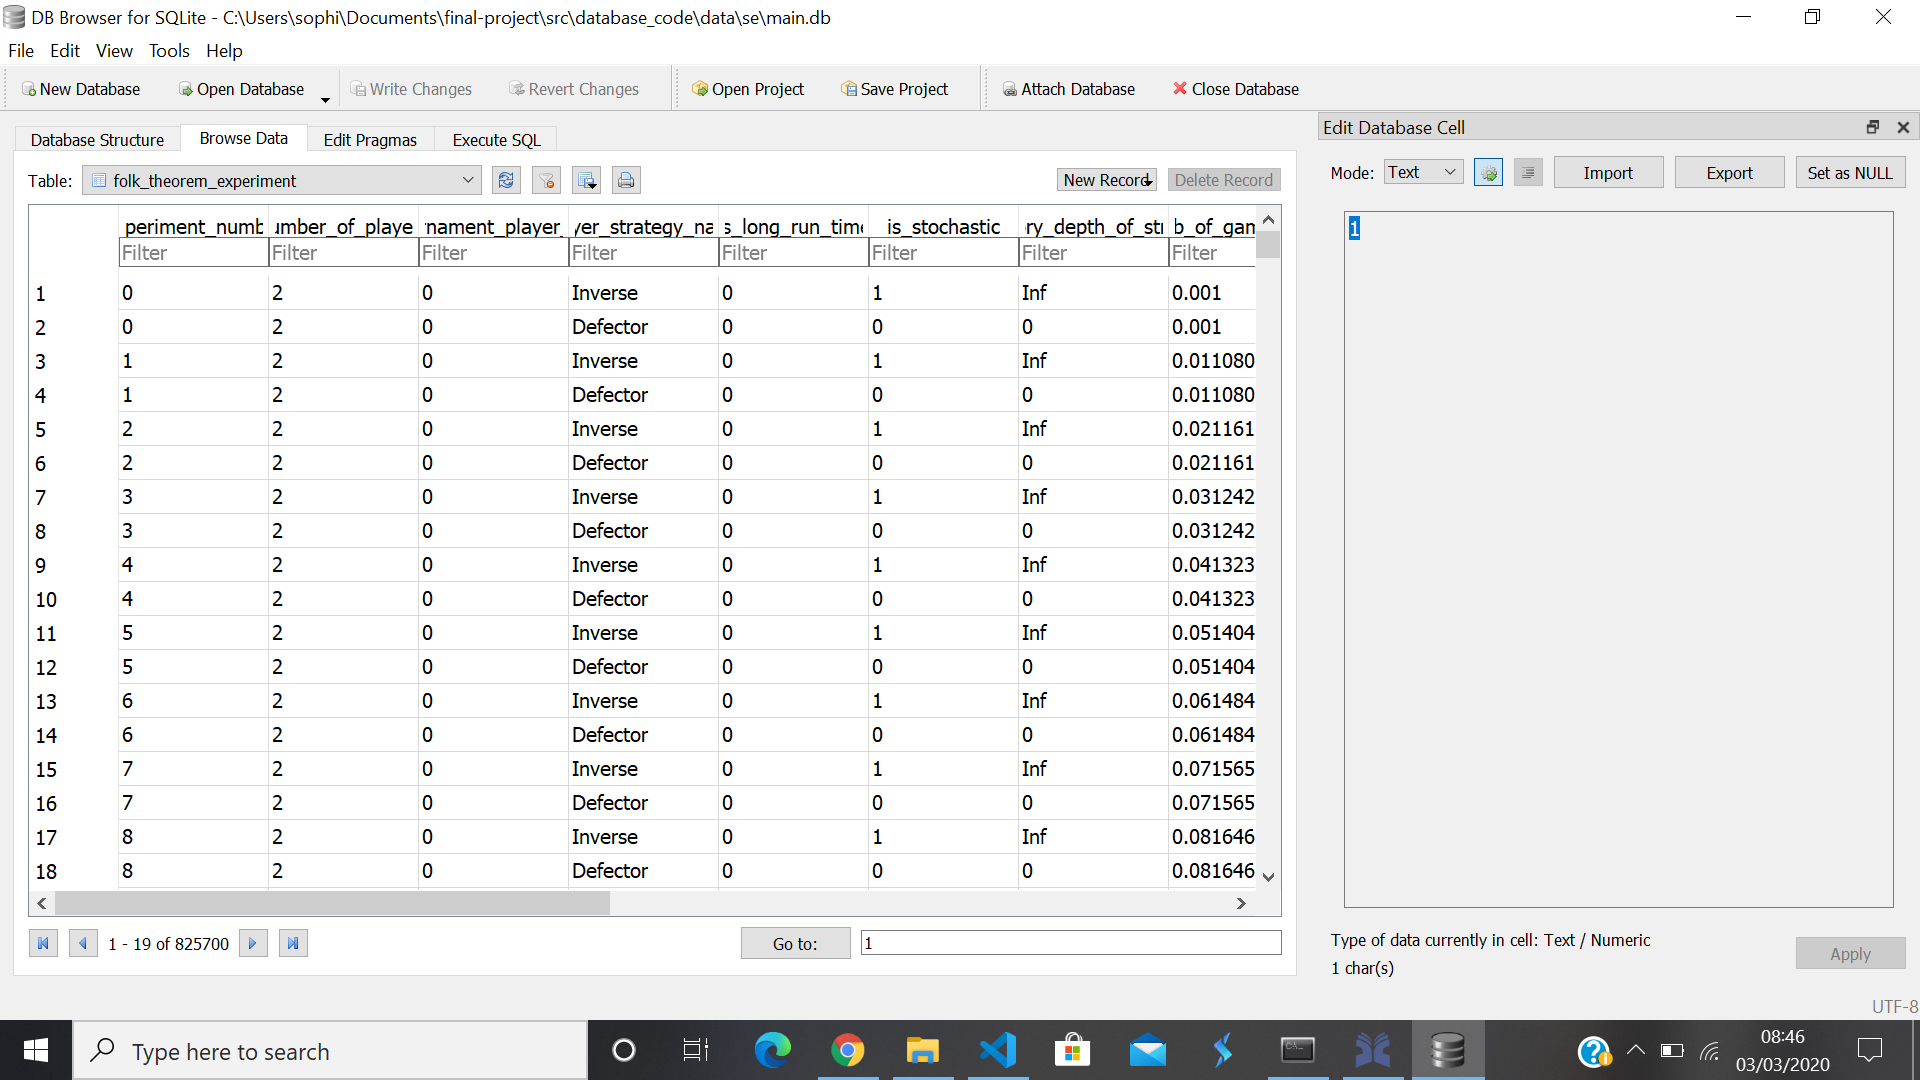
\includegraphics[width=\textwidth]{db_gui_scrnsht.png}
    \caption{DB Browser, a database graphical user interface.}\label{fig:db_browser_scrnsht}
\end{figure}


\section{Software Implementation}\label{sec:Software_Implementation}
There were many potential choices of language for the execution of this 
experiment. However, Python had the added advantage of pre-existing libraries, 
Axelrod~\cite{axelrodproject} and Nashpy~\cite{Nashpy2019}, which enabled running the IPD as well as calculation of the 
Nash equilibria. Thus, Python was used for the collection and analysis of 
data.

Throughout the implementation of this experiment into Python, good software
development principles were followed~\cite{Jimenez2017, Sandve2013, Wilson2014}. Self-documenting code was 
ensured through the careful naming of variables, as well as the use of 
docstrings to fully describe function parameters and usage. Python libraries 
Black~\cite{Langa2019} and Blackbook~\cite{Knight2019a} assisted in improving the readability of the code, through 
formatting according to the guidelines of PEP-8~\cite{Rossum2001}. This gave consistency to all 
code files created during the study. Moreover, modularity was ensured through the creation of several 
smaller functions, focusing on one task. This not only assisted with debugging,
it also allows for future usability of the code in newer developments.

Testing is another key part of software development to guarantee the durability of 
the code. Thus unit tests were implemented, using Pytest~\cite{pytestx.y}, to
assist with the 
identification of bugs in the functions created for data collection. However, 
further work in this area is needed to provide a fully tested program. 
Indeed, from executing the Python library Coverage~\cite{Batchelder2020}, a
coverage of 59\% was identified (for the `experiment\_functions.py' file), 
yielding Table~\ref{tab:cov_scrnsht}. This could be improved through the creation of 
integration tests, between the database and the experiment results, or the 
implementation of functional tests, to confirm the end result of the full 
algorithm.

\begin{table}
    \centering
    \resizebox{\textwidth}{!}{\begin{tabular}{lcccc}
    Module & statements & missing &	excluded & coverage \\
    \midrule
    src/database\_code/\_\_init\_\_.py &	0 &	0 &	0 &	100\% \\
    src/database\_code/experiment\_functions.py &	87 & 36 & 0 & 59\% \\
    src/database\_code/run-experiment-support-enumeration.py & 6 & 6 & 0 & 0\% \\
    src/database\_code/run-experiment-vertex-enumeration.py & 6 & 6 & 0 & 0\% \\
    \midrule
    Total &	99 & 48 & 0 & 52\%
\end{tabular}}
    \caption{A screenshot of the html report produced when utilising Coverage.}\label{tab:cov_scrnsht}
\end{table}

The use of version control is key for keeping track of past changes 
to the system. In this study the software Git~(https://git-scm.com/) was used. This allowed for the 
adaption of code from several different function attempts and, through GitHub~(https://github.com/), 
enabled collaboration between the author and supervisors as seen
in Figure~\ref{fig:github_scrnsht}. The use of GitHub ensured that a back-up copy
of all project files 
were available, should the current system happen to fail. Moreover, it acted as
an intermediate step between the author's laptop and the remote server, which
was used for
running the main experiment (see Section~\ref{sec:Remote_Computing}).

\begin{figure}
    \centering
    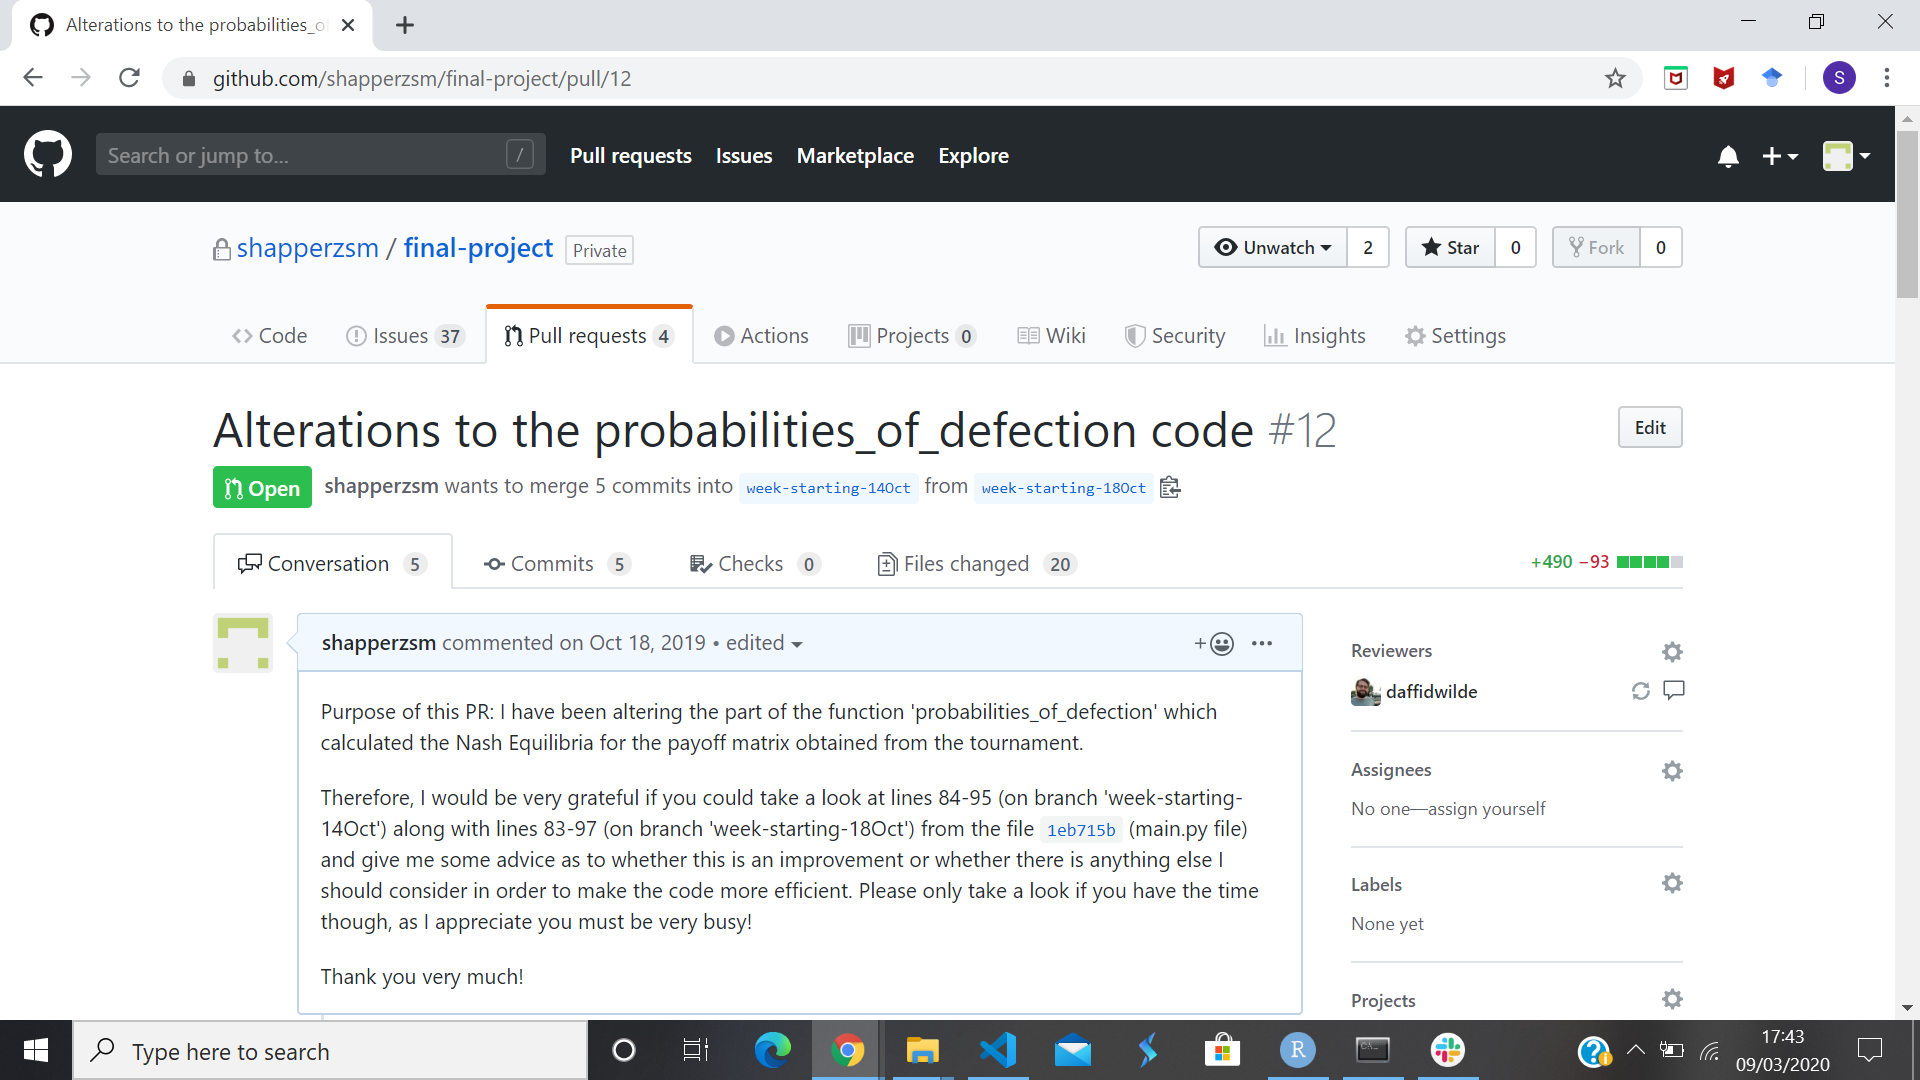
\includegraphics[width=\textwidth]{github_scrnsht.png}
    \caption{A screenshot of a GitHub pull request which allowed for collaboration between supervisors and author.}\label{fig:github_scrnsht}
\end{figure}


\section{Remote Computing}\label{sec:Remote_Computing}
This section describes the execution of the experiments via a remote
computer and the reasons for doing so.

Firstly, due to the volume of data that was planned on being collected, it was
decided that running the data remotely would be ideal, in order to allow the
code to run uninterrupted for several weeks. Thus, Cardiff University School of
Mathematics' computer Siren, a headless server with large storage, was used. However, when a trial was executed,
it was decided that the run time was `quick enough' and hence parallel
processing would not be necessary. Yet, for future runs of the code, parallel
processing is recommended, especially if the player set sizes being trialled are
`large'. See Section~\ref{subsec:Alg_Execution_Times} for an explanation.

\begin{figure}
    \centering
    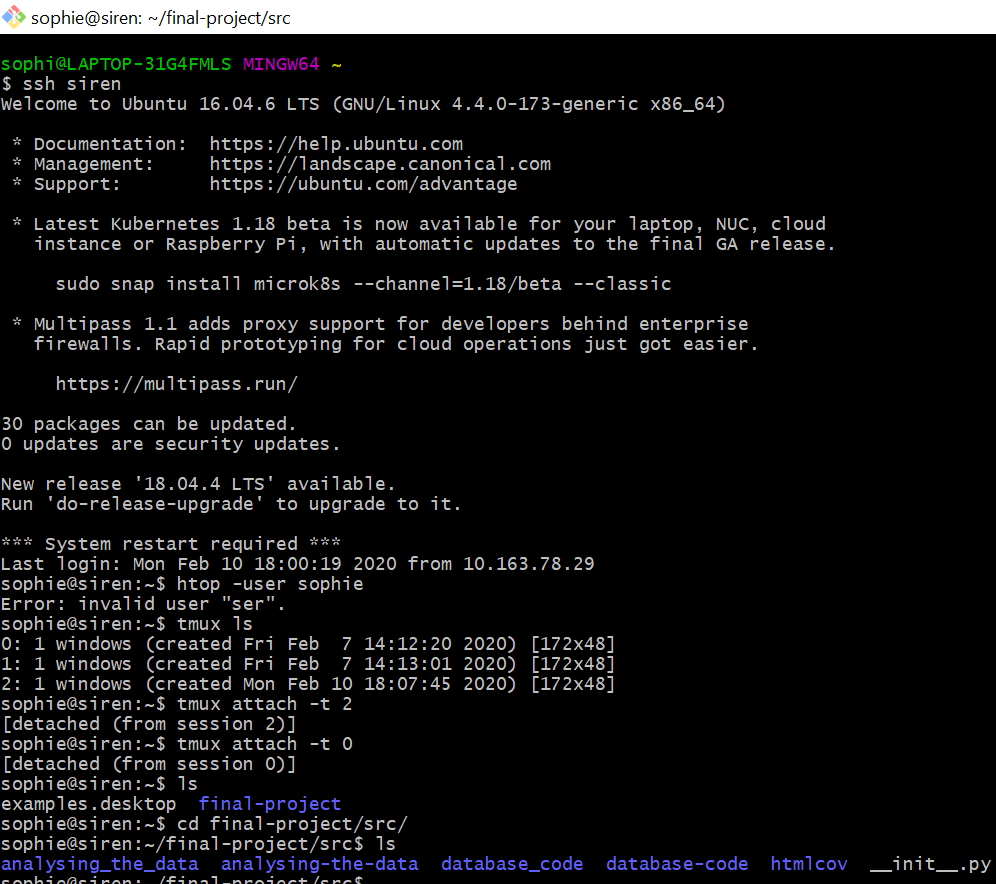
\includegraphics[width=\textwidth]{siren_scrnsht.png}
    \caption{A screenshot of the authors connection to Siren via an SSH tunnel.}\label{fig:siren_scrnsht}
\end{figure}


To connect to Siren, an SSH tunnel was used. An SSH (or Secure Shell) tunnel is
used for sending and receiving network data over an encrypted connection. It adds
a layer of network security, to those applications that do not natively support
encryption, and lowers the risk of interception. For a more detailed description
of SSH, see~\cite{SSH.COM2016}. Figure~\ref{fig:siren_scrnsht} shows the author's
connection to Siren via SSH\@. 


In order for the experiment to keep running, whilst disconnected
from Siren, a terminal emulator was required, as Siren does not have a job
scheduler. Specifically, the terminal multiplexer, TMUX~\cite{Marriott} was used. This allowed
for the creation and execution of several terminals from one screen. Moreover, a
user could detach from a terminal and reattach later without execution being
halted. Figure~\ref{fig:remote_comp}, shows a diagram of how the remote server, ssh tunnel, and user's
laptop, were all in connection.

\begin{figure}
    \centering
    % remote computing diagram
\begin{tikzpicture}
    \draw[dashed] (0,0) rectangle (14,7);
    \draw[blue, thick] (1,2.25) rectangle (4,4.25);
    \node[blue, below] at (2.5, 3.5) {\small author's laptop};
    \draw[green, thick] (8, 1) rectangle (12.5, 5.5);
    \node[green, above] at (12, 6) {\small remote server};
    \draw[orange, dashed] (10.5, 3.5) rectangle (12,5);
    \draw[orange, dashed] (8.5, 3.5) rectangle (10,5);
    \draw[orange, dashed] (10.5, 1.5) rectangle (12,3);
    \draw[orange, dashed] (8.5, 1.5) rectangle (10,3);
    \node[orange, above] at (11,1) {\small TMUX sessions};
    \draw[snake=coil, red, thick, segment aspect=0] (4.5,3.5) -- (7.5, 3.5);
    \draw[snake=coil, red, thick, segment aspect=0] (4.5,2.5) -- (7.5,2.5);
    \node[red, above] at (6, 2.75) {\small ssh tunnel};
\end{tikzpicture}
    \caption{Representation of how the experiments were run remotely. Note, `tmux sessions' correspond to emulators of terminals.}\label{fig:remote_comp}
\end{figure}

Once the experiment was running, the database had to be copied from
Siren in order for analysis to begin. This was also achieved via SSH\@. Note, the code was written in a way
which enabled the results to be written to the database concurrently, after
every tournament. This was done to ensure that, if the system were to break, data
would still have been available and retained within the database. This meant
the database file was almost always `open' resulting in the integrity check
failing once transferred over SSH and an OperationalError in SQLAlchemy. Thus, in
order to to load the database, with no failures, into a Jupyter Notebook, it
needed to be compressed before transferring. This was achieved using the command
line code as seen in Figure~\ref{fig:cmd_code_db}.

\begin{figure}
    \centering
    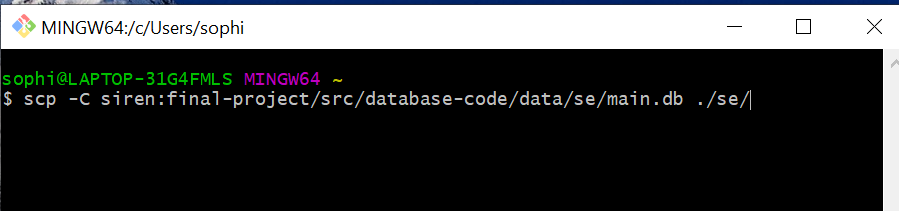
\includegraphics[width=\textwidth]{cmd_line_scrnsht.png}
    \caption{Command line code used to retrieve the database from the remote server.}\label{fig:cmd_code_db}
\end{figure}

\section{Calculating Nash Equilibria}\label{sec:Calculating_Nash_Equilibria}
Recall Nash's Theorem, Theorem~\ref{thm:Nash},
explains that there exists at least one equilibrium in every finite game.
However, it does not indicate how to obtain them. The proof of the theorem
relies on finding the fixed point of the defined mapping but the proof of
Brouwer's Fixed Point Theorem is an existence, and not a constructive, proof.
That is, it does not give a method for obtaining the fixed point. Indeed,
although not NP-complete\footnote{Both finding Brouwer fixed points and Nash
equilibria cannot be NP-complete since existence of a solution is
guaranteed~\cite{NoamNisan2007}. Most problems in the set NP-complete are situations in which
a solution might not exist~\cite{NoamNisan2007}. However,~\cite{papadimitriou1994complexity} has shown that these two
problems belong to a alternative complexity class, PPAD or Polynomial Parity
Argument (Directed case). For a discussion into this, readers are referred to~\cite{papadimitriou1994complexity}.}, finding Brouwer fixed points has been shown to be a 
hard problem~\cite{Hirsch1989,papadimitriou1994complexity}. Thus, defining algorithms which obtain Nash equilibria to
some degree of efficiency has been a large research topic for many years,
particularly in the 2000s. Example papers include~\cite{Bossea,Chen2006,Gilpina,Govindan2003,Kontogiannis2006,Krawczyk2000,Littman2005}. Within the Python Library Nashpy~\cite{axelrodproject}, three
such algorithms have been
implemented: Support Enumeration, Vertex Enumeration and Lemke-Howson. However,
the Lemke-Howson Algorithm will only find \textit{one} equilibria and hence is not
suitable for this study. Therefore the definitions of the first two algorithms,
in the case of a two player game, are provided. Unless specified otherwise, this
section (Section~\ref{sec:Calculating_Nash_Equilibria}) is adapted from~\cite{NoamNisan2007}.


\subsection{Support Enumeration}\label{subsec:Support_Enumeration}
Before stating the method for the support enumeration algorithm, a few extra
theoretical ideas are needed. 

Recall, a \textit{mixed strategy}, \(\sigma \), is a probability distribution
over the pure strategies.

\newpage
\begin{definition}
    The \emph{support} of \(\sigma \) is the set of all pure strategies, \(s_{i}
    \in \sigma \), such that \(s_{i} > 0\). That is, all pure strategies which
    have a positive probability within the mixed strategy.
\end{definition}

\begin{definition}
    A game \(G = (N, {(S_{i})}_{i \in N}, {(u_{i})}_{i \in N})\)
    is called \emph{non-degenerate} if no mixed strategy of support size \(1 \le
    k \le |S_{i}|\) has more than \(k\) pure best responses.
\end{definition}\label{def:non_degen}

For example, consider the following 2-player normal form game:
\begin{equation}
        A = \begin{pmatrix}
                2 & 1 & 0\\
                2 & 0 & 3
        \end{pmatrix}
\end{equation}\label{eqn:degen_game}


In~\eqref{eqn:degen_game}, if the column player was playing the strategy \(\sigma_{2} = (0.2, 0.8,
0)\) then the support is \{strategy1, strategy2\}. Also, observe that, if the
column player picked strategy1 then the row player could choose either their
first or second strategy and hence this game is \textit{degenerate}. 

The method of support enumeration is given in Algorithm~\ref{alg:supp_en}.

\IncMargin{2em}
\begin{algorithm}
    \footnotesize
    \DontPrintSemicolon
    \SetKwInOut{Input}{input}
    \SetKwInOut{Output}{output}

    \Input{A \emph{nondegenerate} two-player normal form game, where \(A, B\)
    are the row and column player's payoff matrices and \(\sigma_{1},
    \sigma_{2}\) are their strategy vectors, respectively.}
    \Output{Every Nash equilibrium of the input game.}
    \For{all \(k = 1, \ldots, \min{\{m, n\}}\)}{
    \For{all support pairs \(I, J\), with \(I \in M, J \in N\) and
    \(|I|=|J|=k\)}{
            Solve \begin{equation}
    \sum_{i \in I}{\sigma_{1i}B_{i,j}} = v, \text{ such that } \sum_{i \in
    I}{\sigma_{1i}} = 1, \sigma_{1i} \ge \textbf{0} \text{ for all } j \in J
            \end{equation}\label{eqn:lin_eqn_1_se} and 
            \begin{equation}
                    \sum_{j \in J}{A_{i, j}\sigma_{2j}} = u, \text{ such that }
                    \sum_{j \ in J}{\sigma_{1i}} = 1, \sigma_{1i} \ge
                    \textbf{0} \text{ for all } i \in I     
            \end{equation}\label{eqn:lin_eqn_2_se}\;
            
            Check the best response conditions \begin{equation}
                \sigma_{1i} > 0 \implies {(A\sigma_{2})}_{i} = \max \{{{(A\sigma_{2})}_{k} | k \in M}\}
            \end{equation} and 
            \begin{equation}
                \sigma_{2j} > 0 \implies {(\sigma_{1}B)}_{j} = \max \{{{(\sigma_{1}B)}_{l} | l \in N}\}
            \end{equation}

        }
    }
    \caption{Support Enumeration}\label{alg:supp_en}
\end{algorithm}
\DecMargin{2em}

Note, in Algorithm~\ref{alg:supp_en}, solutions are not guaranteed to exist for (3.3) and (3.4). In this case, the support does not yield a Nash
equilibrium. 

\subsubsection{An example}
Here the computation of Nash equilibria via support enumeration is considered
for a payoff matrix obtained from a two-player IPD tournament\footnote{Note, the \textit{Defector}'s opponent in this tournament
was stochastic player, \textit{Inverse}. Here, \(p_{e} = 0.0514, ~~ p_{n} = 0\). This game was not identified as degenerate.}. 

Consider the following normal form game:
\begin{equation}
    A = \begin{pmatrix}
        3.000 & 0.829 \\
        1.686 & 1.000 \\
    \end{pmatrix}; ~~~
    B = A^{T}
\end{equation}\label{eqn:supp_en_ex}

Firstly, take \(k = 1\), that is, looking for any pure best responses:
\begin{displaymath}
    A = \begin{pmatrix}
        \underline{3.000} & 0.829 \\
        1.686 & \underline{1.000} \\
    \end{pmatrix} ~~~ B = \begin{pmatrix}
        \underline{3.000} & 1.686 \\
        0.829 & \underline{1.000} \\
    \end{pmatrix}.
\end{displaymath}

Thus, two pairs of pure best responses are visible, giving the following two
Nash equilibria:
\begin{displaymath}
    \sigma = \left \{(1, 0), (1, 0)\right \} \text{   and   } \sigma = \left \{(0, 1), (0, 1)\right \}.
\end{displaymath}

Since this is a two-player game, the only other support that needs checking is
\(I = J = \{1, 2\} \). 

Here, (3.3) and (3.4) become,
\begin{displaymath}
    3\sigma_{r1} + 0.829\sigma_{r2} = 1.686\sigma{r1} + \sigma_{r2} ~~ \text{   and   } ~~ \\
    3\sigma_{c1} + 0.829\sigma_{c2} = 1.686\sigma{c1} + \sigma_{c2}.
\end{displaymath}

Rearranging and checking the constraint \(\sum{\sigma_{r} = 1}, ~~
\sum{\sigma_{c} = 1}\), yields 
\begin{displaymath}
    \sigma_{r1} = \sigma_{c1} = \frac{19}{165} ~~ \text{ and } ~~ \sigma_{r2} = \sigma_{c2} = \frac{146}{165}.
\end{displaymath}

Note, checking the best response condition for two players with the same number
of pure strategies is trivial~\cite{Knight2019b}. However, it is included here for completeness.
\begin{displaymath}
    A\sigma_{c}^{T} = \begin{pmatrix}
        3 & 0.829 \\
        1.686 & 1 \\
    \end{pmatrix} \begin{pmatrix}
        \frac{19}{165} \\
        \frac{146}{165} \\
    \end{pmatrix} = \begin{pmatrix}
        1.079 \\
        1.079 \\
    \end{pmatrix} \text{   and   }
\end{displaymath}

\begin{displaymath}
    \sigma_{r}B = \begin{pmatrix}
        \frac{19}{165} & \frac{146}{165} \\
    \end{pmatrix} \begin{pmatrix}
        3 & 1.686 \\
        0.829 & 1 \\
    \end{pmatrix} = \begin{pmatrix}
        1.079 & 1.079
    \end{pmatrix}
\end{displaymath}

Therefore, the best response condition holds for both players. Hence, the third and final Nash equilibrium is given by:
\begin{displaymath}
    \sigma = \left \{ (\frac{19}{165}, \frac{146}{165}), (\frac{19}{165}, \frac{146}{165})\right \}.
\end{displaymath}


\subsubsection{Advantages and Drawbacks}\label{subsubsec:Adv_and_Drawbacks}
Support enumeration is known to be a robust method for obtaining Nash
equilibria. That is, given a non-degenerate game,
it is guaranteed to return all equilibria and, even in the case of degeneracy,
it will find some equilibria (see Section~\ref{sec:Degeneracy}). However, this method essentially
compares all pairs of supports and thus has an exponential complexity~\cite{Rampersaud2014}. This implies that support enumeration is
computationally expensive and the larger the game, the slower it will become.


\subsection{Vertex Enumeration}\label{subsec:Vertex_Enumeration}
Vertex enumeration is based on a geometric representation of games and hence,
in this section, a brief introduction to this is provided. The reader is
referred to~\cite{NoamNisan2007} for a more detailed approach to this topic.

\begin{definition}
    Let \(A, B\) be \emph{positive} payoff matrices for the row and column
    player; that is, each element \(a_{ij}, b_{ij} > 0\), for all \(i = 1,
    \ldots, M, j = 1, \ldots, N\). Then the row, column
    \textit{best response polytopes}\footnote{In general, a
    \emph{polytope} is defined as a bounded set \( \{z \in \mathbb{R}^{d} |
    Cz^{T} \le q\} \) where \(C\) is a \(k \times d\) matrix and \(z\) is a \(1
    \times d\) vector~\cite{NoamNisan2007}.}, denoted \(P, Q\) are given respectively by
    \begin{equation}
        P = \{x \in \mathbb{R}^{M} | x \ge \textbf{0}, ~ xB \le \textbf{1}\} ~~~
        Q = \{y \in \mathbb{R}^{N} | Ay^{T} \le \textbf{1}, ~ y \ge \textbf{0}\}.
    \end{equation}
    It is assumed that the utility values which appear
    in (3.3) and (3.4) have been normalised
    to 1. This means that the vertices are no longer probabilities and hence
    scaling will be required to find the Nash equilibria. Note, the strictly
    positive payoffs is not a constraint since a constant can be added to each
    with no effect. 
\end{definition}\label{def:best_resp_polytopes}


For example, consider the payoff matrix 

\begin{equation}
    A = \begin{pmatrix}
        1 & 5 \\
        4 & 1
    \end{pmatrix}
\end{equation}\label{eqn:ex_vert_en}

Then the best response polytope, \(P\) here is given by the inequalities:
\begin{center}
    \(
        x_{1} \ge 0, ~~
        x_{2} \ge 0, ~~
        x_{1} + 5x_{2} \le 1, ~~
        4x_{1} + x_{2} \le 1
    \)
\end{center}

which yields the following polytope as given in Figure~\ref{fig:best_resp_polytope}.

\begin{figure}
    \centering
    % best response polytope example
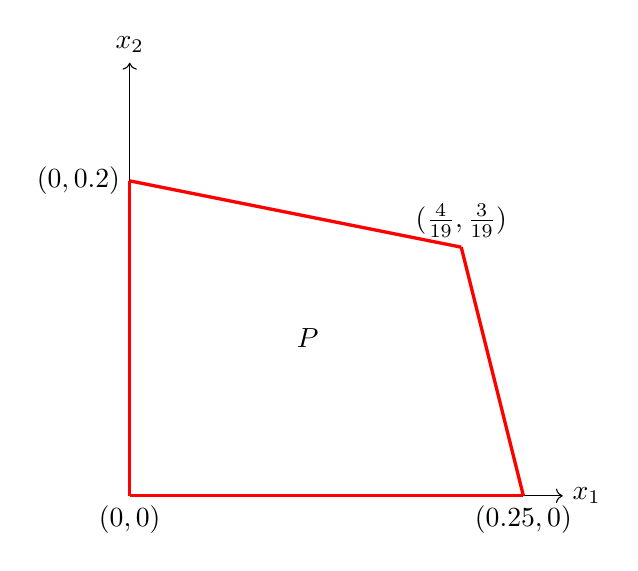
\begin{tikzpicture}
    \draw[->] (0,0) -- (5.5,0) node[right]{$x_{1}$};
    \draw[->] (0,0) -- (0,5.5) node[above]{$x_{2}$};
    \draw[red, very thick] (0,0) -- (5,0);
    \draw[red, very thick] (5,0) -- (80/19,60/19);
    \draw[red, very thick] (0,0) -- (0,4);
    \draw[red, very thick] (80/19,60/19) -- (0,4);
    \node[below] at (0,0) {$(0,0)$};
    \node[below] at (5,0) {$(0.25,0)$};
    \node[left] at (0,4) {$(0,0.2)$};
    \node[above] at (80/19,60/19) {$(\frac{4}{19}, \frac{3}{19})$};
    \node[right] at (2,2) {$P$};
\end{tikzpicture}
    \caption{Best response polytope, \(P\), obtained from the payoff matrix given in~\eqref{eqn:ex_vert_en}.}\label{fig:best_resp_polytope}
\end{figure}

Two algorithms are given, Algorithm~\ref{alg:vertex_lab} `prepares' the polytope
for Algorithm~\ref{alg:vertex_en} which returns the Nash equilibria.

\IncMargin{2em}
\begin{algorithm}
    \footnotesize
    \DontPrintSemicolon
    \SetKwInOut{Input}{input}
    \SetKwInOut{Output}{output}

    \Input{A polytope, \(P \in \mathbb{R}^{n}\).}
    \Output{A labelled-vertex polytope.}
    enumerate each of the defining inequalities of \(P\), \(c_{1}, \ldots,
    c_{k}\) \\
    \For{each vertex \(v_{i} \in P\)}{
        find the inequalities of \(P\) which are \textit{binding} at
        \(v_{i}\), that is the defining equations are equalities.\\

    the label of \(v_{i}\) is given by \( \{c_{i1}, \ldots, c_{il}\} \), where
        \(c_{ij}\) is in the label if and only if equation \(c_{j}\) is binding
        for \(v_{i}\).
    }
    \caption{Vertex Labelling}\label{alg:vertex_lab}
\end{algorithm}
\DecMargin{2em}

A pair of labels \(v_{i} \in P, ~ u_{j} \in Q\) are called \emph{fully labelled}
if every inequality `number' of \(P \cup Q\) appears in either the label of
\(v_{i}\) or the label of \(u_{j}\). Then there is a notion which states that
each fully labelled pair, when normalised, corresponds to a Nash equilibrium.
Note, this does not include the vertex pair \((\textbf{0}, \textbf{0})\) since,
although this is a fully labelled pair, it corresponds to neither opponent playing any strategies. 

\IncMargin{2em}
\begin{algorithm}
    \footnotesize
    \DontPrintSemicolon
    \SetKwInOut{Input}{input}
    \SetKwInOut{Output}{output}

    \Input{Best response polytopes, \(P, Q\), as defined
    in~\ref{def:best_resp_polytopes}, for a \emph{nondegenerate} game.}
    \Output{All Nash equilibria of the corresponding game.}
    \For{each polytope, \(P, Q\)}{
        Execute Algorithm~\ref{alg:vertex_lab}.\\
    \For{each pair of vertices \( \{u_{i}, v_{j}\} \) in \(P, Q\) respectively,
    \textit{except} \((\textbf{0}, \textbf{0})\)}{
        check if they are fully labelled.\\
        \If{they are fully labelled}{
            add to the list of equilibria.
        }\Else{
            continue
        }
    }
    }
    \caption{Vertex Enumeration}\label{alg:vertex_en}
\end{algorithm}
\DecMargin{2em}

\subsubsection{Advantages and Drawbacks}\label{subsubsec:Adv_and_Drawbacks}
Vertex enumeration is more efficient than support enumeration, according
to~\cite{NoamNisan2007}, since there are more supports in a game than there are
vertices. Indeed, consider the example of \(M = N\) where \(M, N\) are the
number of binding inequalities in the best response polytopes, \(P, Q\),
respectively. Using the support enumeration algorithm, approximately \(4^{n}\)
support pairs will need to be observed but, according to the `Upper Bound
Theorem' for polytopes~\cite{Alon1985,Brondsted2012,Seidel1995}, \(P\) and \(Q\) have less than \(2.6^{n}\) vertices.
Thus, given there exists an efficient method for enumerating vertices, this
implies less further computational complexity. However, if the game is
degenerate, this algorithm may not return any Nash equilibria. 

\subsection{Algorithm Execution Timings}\label{subsec:Alg_Execution_Times}
Due to the robustness of the support enumeration, it was decided that this would
be the main method of calculating Nash equilibria. Having said this, timings for
each of the two algorithms were obtained, to see
if their computational times were significantly different. For
the purposes of this trial run, the following parameters were used: 100
tournament repetitions, \(p_{e} = 0.2\) and \(p_{n} = 0\). The results can be
seen in Figure~\ref{fig:timing_exp}.

\begin{figure}
    \centering
    \begin{subfigure}{0.45\textwidth}
        \centering
        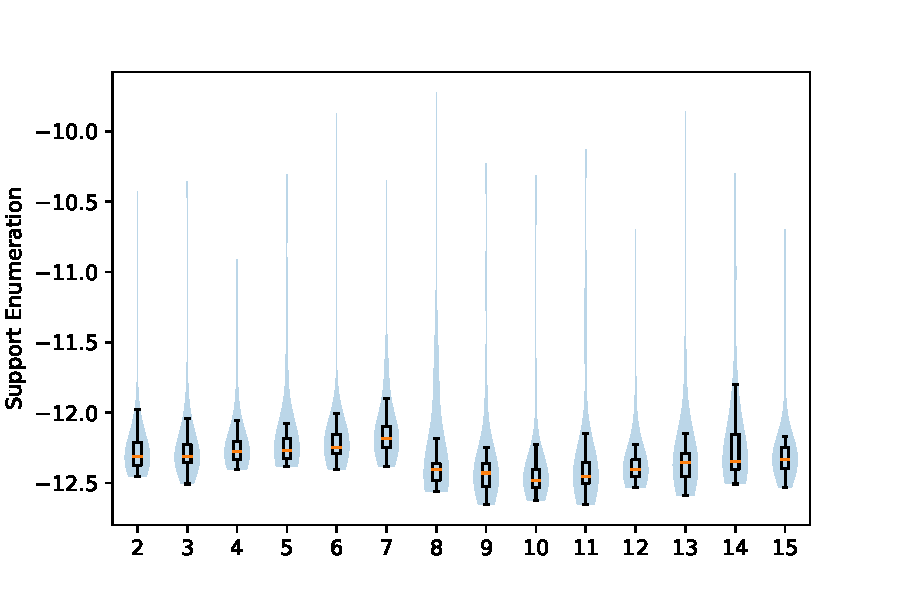
\includegraphics[width=\textwidth]{folk_thm/se_data_time_violinplot.pdf}
        \caption{Timing the support enumeration algorithm.}
    \end{subfigure}
    \hspace{3pt}
    \begin{subfigure}{0.45\textwidth}
        \centering
        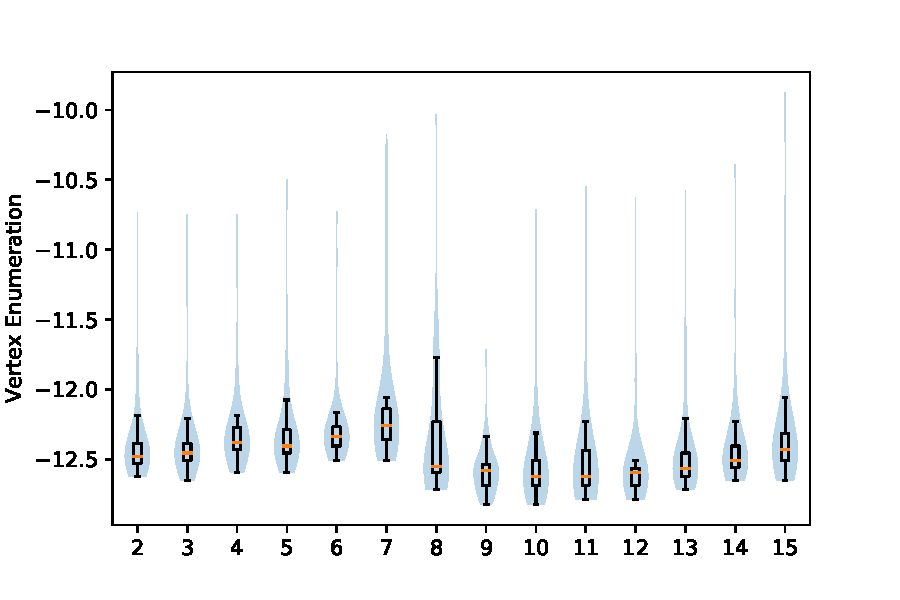
\includegraphics[width=\textwidth]{folk_thm/ve_data_time_violinplot.pdf}
        \caption{Timing the vertex enumeration algorithm.}
    \end{subfigure}
    \caption{Violinplots of the log timings obtained for the experiment and calculation of Nash equilibria using the two algorithms discussed.}\label{fig:timing_exp}
\end{figure}

From Figure~\ref{fig:timing_exp}, it can be seen that there is not a significant
difference in the execution times of the algorithms. Hence, although support
enumeration has a greater computational complexity than vertex enumeration, it
is not going to have any recognisable impact on the number of experiments
executed.


\section{Degeneracy}\label{sec:Degeneracy}
Recall, the definition of non-degeneracy, given in
Definition~\ref{def:non_degen}. This implies a \textit{degenerate} game is one in
which there exists a support of size \(k\) where the number of pure best
responses is greater than \(k\). For example, consider the following payoff
matrix:
\begin{equation}
    A = \begin{pmatrix}
        1 & 4 & 3\\
        0 & 4 & 2
    \end{pmatrix}
\end{equation}
Then, if the column players picks their second strategy (support of size 1),
the row player can pick either of their strategies (that is, two pure best
responses). Thus, this game is degenerate.

Let \(G = (N, {(S_{i})}_{i \in N}, {(u_{i})}_{i \in N})\) be a degenerate game.
Then, recall that support enumeration may not return all Nash equilibria. This
is due to the fact that if solutions to (3.3) and (3.4) of Algorithm~\ref{alg:supp_en} exist, they may not be unique. Indeed, the number of
Nash equilibria in a degenerate game may be infinite~\cite{NoamNisan2007}.
Considering degeneracy in terms of vertex enumeration implies that a vertex of
the best response polytope \(P = \{x \in \mathbb{R}^{M} | x \ge \textbf{0}, ~ xB
\le \textbf{1}\} \) may have more than \(M\) labels leading to a `badly defined'
polytope.

Within the library Nashpy, the algorithms have been implemented such that if
potential degeneracy is identified, for example, by the reasons given above, then
a warning is issued. Thus, in order to retain whether a game is possibly
degenerate, the algorithm was required to `catch' the given warnings. This
was achieved using the code seen in Listing~\ref{ls:warn_code}, with the Python
warnings module.

\begin{listing}
    \begin{minted}[frame = lines, framesep = 2mm, fontsize = \scriptsize, bgcolor = Cornsilk]{python}
    
    with warnings.catch_warnings(record=True) as w:
        warnings.simplefilter("always")

        if support_enumeration is True:
            nash_equilibria = list(game.support_enumeration())

        else:
            highlight_numpy_warning = np.seterr(all="warn")
            nash_equilibria = list(game.vertex_enumeration())

    if len(w) == 0:
        warning_message = None

    else:
        warning_message = str([w[i].message for i in range(len(w))])

    \end{minted}
    \caption{Python code used to `catch' potential degeneracy.}\label{ls:warn_code}
\end{listing}

Note, warnings for potential degeneracy are only highlighted if the
Nash equilibria obtained do not make sense, that is, are not a probability
distribution. On the other hand, it is possible for the algorithm to obtain some
correct Nash equilibria, even if the game is degenerate. This means that, any results, regarding degeneracy of the games, obtained during the
experiment (see Chapter~\ref{ch:Analysis}) need to be inferred with caution. These
are only the games caught by the algorithms in Nashpy and are not necessarily
all of them.

\section{Conclusion}
In this chapter, the creation and execution of the large experiment was
detailed in its entirety. Justifications were given as to why certain methods
and software were used or not. Also, how the Nash equilibria are calculated was
explained, with an example given. Moreover, the potential problems which could
be faced as a result of degeneracy are highlighted.
\chapter{Analyses}

\section{Initial Analysis}

\section{Analysis of the p-Threshold}

\subsection{Effects of Stochastic Players}

\subsection{Effects of Noise}

\subsection{Effects of Degeneracy}

\subsection{Multivariate Data Analysis}
\chapter{Conclusions and Recommendations}\label{ch:Conclusions}
This project looked into the Folk Theorem for the IPD and, in particular, at the
game-ending probabilities for which defection is no longer rational. The three
aims of the study, as given in Chapter~\ref{ch:Introduction}, are restated here for
convenience:

\begin{enumerate}
    \item To provide a review of past and present literature already published in
    the field of folk theorems;
    
    \item To develop a program which executes a large experiment involving
    tournaments of the IPD with differing environments to obtain
    graphs similar to those in Figure~\ref{fig:CW_plots}; and
    
    \item To perform analyses on where the \(p\)-thresholds seem to lie and
    whether it is affected by the change in the number of players, levels of
    standard PD noise, etc.
\end{enumerate}

Therefore, in this chapter, a brief section discussing the results of each aim
is provided. Then, a few shortcomings of the project are mentioned and areas in
which the research could be expanded further are highlighted.

\section{Conclusions}\label{sec:Conclusions}
In this section, each aim is explored with regards to results found and how well they were addressed. Overall, the first two aims were
successfully achieved. A well rounded knowledge in the recent research of
folk theorems was obtained and a successful experiment carried out. However,
maximal results were not obtained for the final aim due to time limitations and
the non-triviality of degeneracy.

\subsection{Aim 1: Reviewing the Literature}\label{subsec:Aim_1_concl}
The first aim was addressed in Chapter~\ref{ch:Lit_Review}. Here, a literature
search on ``folk theorem'' yielded a vast range of results which spanned the
last fifty years. It was discussed that the true origin of the `folk theorem' is
unknown however its statement and proofs appear in written work since the 1970s.
These papers focused on infinitely repeated games with subgame perfect
equilibria. Following this, many generalisations and refinements of the folk
theorem were explored. Varying types of games, for which folk theorems have been
considered, were discussed. These included: games with complete information,
games with imperfect private monitoring and games with communication, among
others. Within these papers, it was also discovered that other equilibria
(besides the more common subgame perfect equilibria) have been considered. Some
examples are: sequential equilibria, belief-free equilibria and type-k
equilibria. Throughout, there appeared to be two main assumptions required for a
folk theorem to exist. These were full dimensionality and the number of
signals in proportion to the number of actions. Since these assumptions are restricting, a few papers have attempted to find situations in which they
can be weakened whilst still obtaining a folk theorem. In contrast, an
area of research has developed which shows the instability of equilibria and
the violation of folk theorems. The chapter is concluded by a discussion on
recent applications of the folk theorem to computing, multi-agent systems and
quantum transportation. Finally, to the best of the author's knowledge, no folk
theorem experiments, of the same size as executed in this study, have been
computed before.

\subsection{Aim 2: Software Development}\label{subsec:Aim_2_concl}
Chapter~\ref{ch:Methods} discusses the set-up and execution of the IPD experiment
referred to in Aim 2. This included justifications for the use of certain
software and methods, as well as a detailed view of the data collection
algorithm. Within this, reasons were given on why the particular attributes
of the tournaments were collected. Following this, an exploration into the
file types available for data collection was provided. After considering
the advantages and drawbacks, it was decided that a binary file, in particular a
relational database file, would be the most appropriate. The chapter then
continues with an explanation of the software implementation of
the aforementioned algorithm. It provides details on how good software
development principles were followed and on the programs utilised. For a more
detailed overview, which is not as involved as the chapter, see
Chapter~\ref{ch:Comp_Report} in the Appendix. The
main experiment was executed remotely over a few weeks and how this was
achieved is explained here. Following this, how to compute the Nash equilibria
and the notion of degeneracy were addressed. Out of the three algorithms: Support
Enumeration, Vertex Enumeration and Lemke-Howson; it was decided that Support
Enumeration would be the method used for calculating Nash equilibria, due to
its robustness. The execution timings of each algorithm were also explored but
did not yield any significant differences. To conclude, the difficulties which
could be faced due to degeneracy were briefly acknowledged and possible
solutions discussed.

\subsection{Aim 3: Analysing the Thresholds}\label{subsec:Aim_3_concl}
The final aim, regarding the analysis of \(p\)-thresholds, was addressed in
Chapter~\ref{ch:Analysis}. Firstly, an initial analysis identified the main `shapes' of the graphs obtained and detailed the summary
statistics. This included looking at characteristics of the strategies, as well
as the number of equilibria obtained from each tournament. The majority of
strategies chosen were deterministic - this is because of the ratio between
deterministic and stochastic strategies implemented in the Axelrod library. When
analysing the thresholds, the minimum, mean, median and maximum
values of the \(p\)-threshold were taken, due to varying sources of noise
obscuring a clear threshold. Here, the focus was on the effects of the number
of players and standard PD noise. However, this was
concluded as a non-trivial task due to the difficulty of identifying degenerate
games and the many sources of noise. As a
result of this, significant conclusions were unable to be drawn with the
obtained plots not revealing many trends. Thus, suggestions are
provided on how further work regarding this study could reveal more significant
information. These are restated in Section~\ref{sec:Recommendations}. In
conclusion however, the experiment was successful in providing clear
visualisations for the folk theorem and it gives insight into a wide range of
directions for future research.

\section{Limitations}\label{sec:Limitations}
In this section a few shortcomings of the study are highlighted along
with justifications.

Firstly, this project included a very large empirical study on the folk theorem.
This required the development and implementation of an algorithm.
Inevitably, to ensure the functions were
accurate, clear and gave the required information, a significant amount of time
was taken. Therefore, one of the main
drawbacks was the time constraint of completing the project. Indeed, after the
successful implementation of the data collection algorithm into Python, there
was a certain time frame before analysis could start. This was to ensure enough data had
been collected. The analysis then took a portion of the time,
especially due to the data's non-triviality mentioned previously.

As a result of this, the amount of data collected was insufficient for a
large-scale statistical analysis on extremely random data. Also, the
parameters used in the algorithm were restricted by this. Only 500
repetitions of each tournament were performed but this was only able to
`stabilise' some of the payoff matrices. The rest resulted in
threshold graphs which were less clear. Thus, higher repetitions were needed but
unrealistic for the given time-frame. Moreover, the eighteen strategies
classified as `long-run' had to be omitted but, in an ideal situation, they
would have been included to obtain more information.

Furthermore, the analysis carried out only briefly considered some of
the potential environmental effects on the \(p\)-threshold. The
`randomness' of the data meant that trends were hard to infer and key
conclusions could not be drawn. Ideally, further environmental
changes, in addition to number of players and level of standard PD noise, would
have been discussed. Another factor which could have improved the situation, but
had to be omitted due to time, was the packaging of the code. Creating a fully
working Python package, with all the required functions implemented, may have
improved the remote computing stage.

Finally, degeneracy was a major limitation due to its uncertainty. Nashpy only
identifies potential degeneracy if the equilibria are `strange'. That is, if the algorithm
detects division by zero or non-probability distributions, for example. Indeed, some
games may still be degenerate even if equilibria are identified.
This implies that discussions regarding degeneracy in
Chapter~\ref{ch:Analysis} assume that Nashpy can
detect all degeneracy, which is unrealistic.

\section{Recommendations}\label{sec:Recommendations}
Throughout this study, many interesting questions have been raised as potential
directions for future work. Hence, in this section, recommendations on how this
research could be extended, to provide more insightful results, are given.

Firstly, during analysis (Chapter~\ref{ch:Analysis}), a significant proportion
of the graphs showed no \(p\)-threshold, appearing constant at zero or one.
This indicates that the threshold must lie in the intervals (0, 001) or (0.999,
1), implying the precision level was not fine enough. Therefore, it is suggested
that these tournaments are rerun, within these intervals, using a greater
precision to obtain more information. Also, an analysis of the
strategies involved and values of standard PD noise might provide a
clearer insight into reasons for this. Moreover, re-running the whole
experiment, with a finer precision could yield
more accurate thresholds.

In order to explore the effects of stochastic players on the threshold, it is
recommended that tournament sets which contain stochastic
players are rerun without them. If the threshold is different, this could indicate that stochasticity does indeed have an effect.

It is highly recommended that a separate run of the experiment is performed,
using vertex enumeration to calculate the equilibria. This could then be used in comparison
with the support enumeration data to check the reliability of the results obtained. However, care is needed when implementing vertex
enumeration as it is less robust, (see Chapter~\ref{ch:Methods}).
Furthermore, increasing the number of tournament repetitions is suggested to
observe whether clearer \(p\)-thresholds are obtained.

Regarding multivariate data analysis of this large empirical study, it may be
insightful to perform a regression or clustering algorithm. This is motivated by
the possibility of being able to approximately predict the \(p\)-threshold of a
tournament by its characteristics: strategies, level of standard PD noise etc.
Finally, the experiment could potentially be extended to consider the different
`types' of folk theorem discussed in Chapter~\ref{ch:Lit_Review}. 



\addcontentsline{toc}{chapter}{References}
\printbibliography[title=References]

\begin{appendices}
	\chapter{APPENDIX A TITLE}



\chapter{APPENDIX B TITLE}


% etc.

\end{appendices}

\end{document}